\section{Experimentos y análisis de resultados}
	
	\subsection{Procedimiento de desarrollo de la práctica}
	
	\paragraph{}Para realizar la práctica, se ha optado por implementar las heurísticas propuestas en el lenguaje de programación \textsc{Java}. El ejecutable que se entrega junto a este documento ha sido compilado bajo \textsc{ Apache NetBeansIDE 12.0}.
	
	\subsubsection{Equipo de pruebas}
	
	\paragraph{}Los resultados de las heurísticas han sido obtenidos en el siguiente equipo:
	
		\begin{itemize}
			
			\item Host:
			\item S.O:
			\item Kernel:
			\item CPU:
			\item GPU:
			\item GPU:
			\item Memoria RAM :
			
		\end{itemize}

	\subsubsection{Manual de usuario}
	
		\paragraph{}Para ejecutar el software asegúrese de que el archivo .jar proporcionado se ubica en el mismo directorio que la carpeta \emph{archivos}. 
		
		\paragraph{}Cuando se muestre la GUI, podrá seleccionar la heurística que desee mediante el botón correspondiente. Una vez empiece la ejecución de una heurística no sera posible seleccionar otra hasta que finalice su ejecución. Los resultados finales se mostrarán en el cuadro de texto, a su vez, se generan los log correspondientes a cada archivo y semilla en la carpeta Log.
	
		\begin{figure}[H]
		
			\centering
			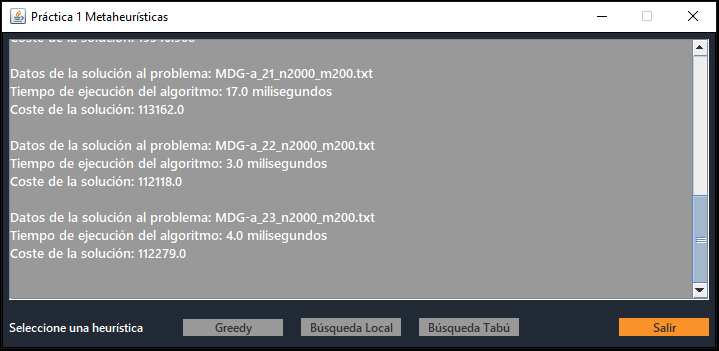
\includegraphics[scale=0.4]{img/GUI}
			\caption{GUI}
		
		\end{figure}
	
	\subsection{Parámetros de los algoritmos}
	
		\subsubsection{Sistema de Colonias de Hormigas}

		\paragraph{}Para regular el comportamiento del Sistema de Colonias de Hormigas, se han definido los siguientes parámetros en el archivo de configuración:
		
		\begin{itemize}
			
			\item Iteraciones:  Número máximo de iteraciones realizadas por el algoritmo principal, valor por defecto: 10.000.
			\item Número de hormigas: Número de hormigas pertenecientes a cada colonia generada en cada iteración, valor por defecto: 10.
			\item Q0: Probabilidad de no elegir directamente el candidato que mayor coste aporta a la hormiga en la regla de la transición, valor por defecto: 0,95.
			\item Beta: Exponente aplicado al coste de los arcos en las fórmulas de la regla de la transición, valores por defecto: 1 y 2.
			\item Alfa: Exponente aplicado a la feromona de los arcos en las fórmulas de la regla de la transición, valores por defecto: 1 y 2.
			\item Rho: Constante aplicada en la fórmula de la evaporación global de feromona, valor por defecto: 0,1.
			\item Phi: Constante aplicada en la fórmula de la evaporación local de feromona, valor por defecto: 0,1.
			\item Delta: Porcentaje de restricción aplicado sobre la lista de candidatos total de una hormiga, valor por defecto: 0,75.
			
		\end{itemize}
	\subsubsection{Semillas}
	
	\paragraph{}Para la generación de números pseudoaleatorios se utiliza una semilla previamente definida en el archivo de configuración, en este caso es 77356084. Esta semilla se va rotando en las 5 iteraciones de cada archivo.
	
	
	\paragraph{} 77356084 $\rightarrow$ 73560847 $\rightarrow$ 35608477  ...
	
	
	\subsection{Análisis de los resultados}
	
		\subsubsection{SCH con $\alpha$ = 1, $\beta$ =1}
		
		\paragraph{}De la experimentación realizada, obtenemos las siguientes tablas, correspondientes al S.C.H. con $\alpha$ = 1 y $\beta$ = 1:
		
		\begin{table}[H]
			\begin{center}
				\begin{tabular}{| c | c | c | c | c | c | c |}
					\hline
					\multicolumn{7}{ |c| }{SCH $\alpha$ = 1, $\beta$ =1} \\ \hline
					& \multicolumn{2}{ |c| }{GKD-c\_1\_n500\_m50} & \multicolumn{2}{ |c| }{GKD-c\_2\_n500\_m50} & \multicolumn{2}{ |c| }{GKD-c\_3\_n500\_m50} \\ \hline
					Ejecución & Coste & Tiempo & Coste & Tiempo & Coste & Tiempo \\ \hline
					1 &19447,05 & 86283 & 19677,01 & 85025 & 19525,05 & 85636\\
					2 &19460,39 & 85767 & 19674,26 & 85178 & 19523,76 & 85188\\
					3 &19462,50	& 87097 & 19670,57 & 85011 & 19519,77 & 85287\\
					4 &19458,63	& 86364 & 19661,08 & 85106 & 19523,81 & 85303\\
					5 &19462,67 & 86277 & 19674,56 & 85214 & 19531,01 & 85232\\ \hline
					Media & -0,14\% & 86357,60 & -0,15\% & 85106,80 & -0,12\% & 85329,20\\ \hline
					Devs. típica & 0,03\% & 476,35 & 0,03\% & 90,04 & 0,02\% & 177,47 \\ \hline
				\end{tabular}
				\caption{Resultados GKD}
				\label{tab:tabalfa1beta1GKD}
			\end{center}
		\end{table} 
		
		
		\begin{table}[H]
			\begin{center}
				\begin{tabular}{| c | c | c | c | c | c | c |}
					\hline
					\multicolumn{7}{ |c| }{SCH $\alpha$ = 1, $\beta$ =1} \\ \hline
					& \multicolumn{2}{ |c| }{SOM-b\_11\_n300\_m90} & \multicolumn{2}{ |c| }{SOM-b\_12\_n300\_m120} & \multicolumn{2}{ |c| }{SOM-b\_13\_n400\_m40} \\ \hline
					Ejecución & Coste & Tiempo & Coste & Tiempo & Coste & Tiempo\\\hline
					1 &20662 & 167862 & 35800 & 263791 & 4630 & 53726\\
					2 &20658 & 167622 & 35793 & 264292 & 4626 & 53753\\
					3 &20645 & 167410 & 35780 & 263622 & 4646 & 53726\\
					4 &20623 & 167560 & 35828 & 263551 & 4631 & 53832\\
					5 &20634 & 167525 & 35776 & 263251 & 4629 & 54074\\\hline
					Media &-0,48\% & 167595,80 & -0,24\% & 263701,40 & -0,55\% & 604,40\\ \hline
					Devs. típica & 0,08\% & 167,70 & 0,06\% & 383,61 & 0,17\% & 7,44 \\ \hline
				\end{tabular}
				\caption{Resultados SOM}
				\label{tab:tabalfa1beta1SOM}
			\end{center}
		\end{table} 
		
		\begin{table}[H]
			\begin{center}
				\begin{tabular}{| c | c | c | c | c | c | c |}
					\hline
					\multicolumn{7}{ |c| }{SCH $\alpha$ = 1, $\beta$ =1} \\ \hline
					& \multicolumn{2}{ |c| }{MDG-a\_21\_n2000\_m200} & \multicolumn{2}{ |c| }{MDG-a\_22\_n2000\_m200} & \multicolumn{2}{ |c| }{MDG-a\_23\_n2000\_m200}\\\hline
					Ejecución & Coste & Tiempo & Coste & Tiempo & Coste & Tiempo\\\hline
					1 &113383,00 & 600256,00 & 113153,00 & 600090,00 & 113132,00 & 600032,00\\
					2 &113539,00 & 600065,00 & 113180,00 & 600185,00 & 113110,00 & 600298,00\\
					3 &113368,00 & 600107,00 & 113439,00 & 600184,00 & 113088,00 & 600292,00\\
					4 &113483,00 & 600283,00 & 113232,00 & 600161,00 & 113064,00 & 600116,00\\
					5 &113307,00 & 600149,00 & 113258,00 & 600124,00 & 113085,00 & 600223,00\\\hline
					Media &-0,74\% & 600172,00 & -0,94\% & 600178,80 & -0,90\% & 6000192,20\\ \hline
					Devs. típica & 0,08\% & 94,31 & 0,10\% & 41,14 & 0,02\% & 115,73 \\ \hline
				\end{tabular}
				\caption{Resultados MDG}
				\label{tab:tabalfa1beta1MDG}
			\end{center}
		\end{table}
		
		\paragraph{} Como puede observarse en los resultados, el algoritmo exhibe un comportamiento robusto, manteniendo las desviación típica de los resultados por debajo del 0,10\% en casi todos los archivos estudiados, a excepción de dos. En todo caso la mayor desviación típica alcanzada no sobrepasa el 0,20\%. Si evaluamos la calidad de las soluciones obtenidas respecto a costes, el algoritmo es incapaz de encontrar los óptimos globales con los parámetros anteriormente descritos.
		
		\paragraph{} En lo referente a tiempos, el algoritmo consigue ejecutar las iteraciones objetivo antes de los 600 segundos para las instancias pequeñas y medianas. No es el caso de las instancias de datos más grandes, dónde el algoritmo finaliza su ejecución en torno las 2000 iteraciones, sin sobrepasar las 3.000 iteraciones en ningún caso,para los archivos MDG. 
		
		\subsubsection{SCH con $\alpha$ = 2, $\beta$ =1}
		
		\paragraph{}De la experimentación realizada, obtenemos las siguientes tablas, correspondientes al S.C.H. con $\alpha$ = 2 y $\beta$ = 1:
		
		\begin{table}[H]
			\begin{center}
				\begin{tabular}{| c | c | c | c | c | c | c |}
					\hline
					\multicolumn{7}{ |c| }{SCH $\alpha$ = 2, $\beta$ =1} \\ \hline
					& \multicolumn{2}{ |c| }{GKD-c\_1\_n500\_m50} & \multicolumn{2}{ |c| }{GKD-c\_2\_n500\_m50} & \multicolumn{2}{ |c| }{GKD-c\_3\_n500\_m50} \\ \hline
					Ejecución & Coste & Tiempo & Coste & Tiempo & Coste & Tiempo \\ \hline
					1 &19474,14	& 75409,00 & 19690,75 & 74542,00 & 19531,98 & 74963,00\\
					2 &19467,52 & 74773,00 & 19684,14 & 74459,00 & 19530,92 & 75088,00\\
					3 &19470,50	& 75609,00 & 19676,87 & 74610,00 & 19531,78 & 75081,00\\
					4 &19470,51 & 74761,00 & 19684,42 & 74624,00 & 19528,11 & 74778,00\\
					5 &19470,31 & 74776,00 & 19685,35 & 74741,00 & 19535,05 & 74920,00\\ \hline
					Media &-0,07\% & 75065,60 & -0,09\% & 74595,20 & -0,08\% & 74966,00\\ \hline
					Devs. típica & 0,01\% & 410,94 & 0,03\% & 104,51 & 0,01\% & 128,04\\ \hline
				\end{tabular}
				\caption{Resultados GKD}
				\label{tab:tabalfa2beta1GKD}
			\end{center}
		\end{table} 
		
		
		\begin{table}[H]
			\begin{center}
				\begin{tabular}{| c | c | c | c | c | c | c |}
					\hline
					\multicolumn{7}{ |c| }{SCH $\alpha$ = 2, $\beta$ =1} \\ \hline
					& \multicolumn{2}{ |c| }{SOM-b\_11\_n300\_m90} & \multicolumn{2}{ |c| }{SOM-b\_12\_n300\_m120} & \multicolumn{2}{ |c| }{SOM-b\_13\_n400\_m40} \\ \hline
					Ejecución & Coste & Tiempo & Coste & Tiempo & Coste & Tiempo\\\hline
					1 &20659,00 & 137093,00 & 35850,00 & 208580,00 & 4624,00 & 45791,00\\
					2 &20680,00 & 136936,00 & 35841,00 & 208674,00 & 4649,00 & 45878,00\\
					3 &20676,00 & 136880,00 & 35854,00 & 208779,00 & 4656,00 & 45488,00\\
					4 &20685,00 & 137012,00 & 35855,00 & 209401,00 & 4658,00 & 44994,00\\
					5 &20670,00 & 136576,00 & 35853,00 & 208708,00 & 4658,00 & 45268,00\\ \hline
					Media &-0,33\% & 136899,40 & -0,08\% & 208828,40 & -0,19\% & 45483,80\\ \hline
					Devs. típica & 0,05\% & 197,78 & 0,02\% & 328,01 & 0,31\% & 366,15\\ \hline
				\end{tabular}
				\caption{Resultados SOM}
				\label{tab:tabalfa2beta1SOM}
			\end{center}
		\end{table} 
		
		\begin{table}[H]
			\begin{center}
				\begin{tabular}{| c | c | c | c | c | c | c |}
					\hline
					\multicolumn{7}{ |c| }{SCH $\alpha$ = 2, $\beta$ =1} \\ \hline
					& \multicolumn{2}{ |c| }{MDG-a\_21\_n2000\_m200} & \multicolumn{2}{ |c| }{MDG-a\_22\_n2000\_m200} & \multicolumn{2}{ |c| }{MDG-a\_23\_n2000\_m200}\\\hline
					Ejecución & Coste & Tiempo & Coste & Tiempo & Coste & Tiempo\\\hline
					1 &113803,00 & 600034,00 & 113790,00 & 600104,00 & 113361,00 & 600223,00\\
					2 &113662,00 & 600153,00 & 113463,00 & 600130,00 & 113594,00 & 600144,00\\
					3 &113831,00 & 600100,00 & 113649,00 & 600142,00 & 113516,00 & 600155,00\\
					4 &113906,00 & 600218,00 & 113653,00 & 600086,00 & 113369,00 & 600057,00\\
					5 &113879,00 & 600192,00 & 113646,00 & 600054,00 & 113505,00 & 600036,00\\ \hline
					Media &-0,39\% & 600139,40 & -0,60\% & 600103,20 & -0,57\% & 600123,00\\ \hline
					Devs. típica & 0,08\% & 73,81 & 0,10\% & 35,15 & 0,09\% & 76,47 \\ \hline
				\end{tabular}
				\caption{Resultados MDG}
				\label{tab:tabalfa2beta1MDG}
			\end{center}
		\end{table}
	
		\paragraph{} Como puede observarse en los resultados, el algoritmo exhibe un comportamiento robusto, manteniendo las desviación típica de los resultados por debajo del 0,10\% en casi todos los archivos estudiados, a excepción de dos. En todo caso la mayor desviación típica alcanzada es de un 0,31\%. Si evaluamos la calidad de las soluciones obtenidas respecto a costes, el algoritmo solo es capaz de encontrar el óptimo global para el archivo SOM-b\_12\_n300\_m120 con los parámetros anteriormente descritos.
		
		\paragraph{} En lo referente a tiempos, el algoritmo consigue ejecutar las iteraciones objetivo antes de los 600 segundos para las instancias pequeñas y medianas. No es el caso de las instancias de datos más grandes, dónde el algoritmo finaliza su ejecución en torno las 2.000 iteraciones, sin sobrepasar las 3.000 iteraciones en ningún caso, para los archivos MDG.
		
		\subsubsection{SCH con $\alpha$ = 1, $\beta$ =2}
		
		\paragraph{}De la experimentación realizada, obtenemos las siguientes tablas, correspondientes al S.C.H. con $\alpha$ = 1 y $\beta$ = 2:
	
		\begin{table}[H]
			\begin{center}
				\begin{tabular}{| c | c | c | c | c | c | c |}
					\hline
					\multicolumn{7}{ |c| }{SCH $\alpha$ = 1, $\beta$ =1} \\ \hline
					& \multicolumn{2}{ |c| }{GKD-c\_1\_n500\_m50} & \multicolumn{2}{ |c| }{GKD-c\_2\_n500\_m50} & \multicolumn{2}{ |c| }{GKD-c\_3\_n500\_m50} \\ \hline
					Ejecución & Coste & Tiempo & Coste & Tiempo & Coste & Tiempo \\ \hline
					1 &19458,15 & 77625,00 & 19671,65 & 74997,00 & 19524,13 & 75122,00\\
					2 &19464,52 & 75155,00 & 19674,24 & 75196,00 & 19517,79 & 75309,00\\
					3 &19461,56	& 75467,00 & 19672,58 & 75163,00 & 19512,71 & 75040,00\\
					4 &19453,08	& 76501,00 & 19663,09 & 75141,00 & 19519,27 & 75298,00\\
					5 &19455,44 & 75050,00 & 19671,50 & 75515,00 & 19513,44 & 75086,00\\ \hline
					Media & -0,14\% & 75959,60 & -0,16\% & 75202,40 & -0,15\% & 75171,00\\ \hline
					Devs. típica & 0,02\% & 1093,63& 0,02\% & 190,57 & 0,02\% & 124,46\\ \hline
				\end{tabular}
				\caption{Resultados GKD}
				\label{tab:tabalfa1beta2GKD}
			\end{center}
		\end{table} 
		
		
		\begin{table}[H]
			\begin{center}
				\begin{tabular}{| c | c | c | c | c | c | c |}
					\hline
					\multicolumn{7}{ |c| }{SCH $\alpha$ = 1, $\beta$ =1} \\ \hline
					& \multicolumn{2}{ |c| }{SOM-b\_11\_n300\_m90} & \multicolumn{2}{ |c| }{SOM-b\_12\_n300\_m120} & \multicolumn{2}{ |c| }{SOM-b\_13\_n400\_m40} \\ \hline
					Ejecución & Coste & Tiempo & Coste & Tiempo & Coste & Tiempo\\\hline
					1 &20622,00 & 139098,00 & 35778,00 & 213206,00 & 4623,00 & 47794,00\\
					2 &20642,00 & 138657,00 & 35788,00 & 213358,00 & 4625,00 & 47931,00\\
					3 &20626,00 & 139174,00 & 35801,00 & 213563,00 & 4645,00 & 47870,00\\
					4 &20630,00 & 139116,00 & 35798,00 & 213505,00 & 4628,00 & 48003,00\\
					5 &20659,00 & 139407,00 & 35777,00 & 213245,00 & 4630,00 & 48161,00\\\hline
					Media &-0,52\% & 139090,40 & -0,26\% & 213375,40 & -0,60\% & 47951,80\\ \hline
					Devs. típica & 0,07\% & 271,93 & 0,03\% & 156,52 & 0,19\% & 140,01\\ \hline
				\end{tabular}
				\caption{Resultados SOM}
				\label{tab:tabalfa1beta2SOM}
			\end{center}
		\end{table} 
		
		\begin{table}[H]
			\begin{center}
				\begin{tabular}{| c | c | c | c | c | c | c |}
					\hline
					\multicolumn{7}{ |c| }{SCH $\alpha$ = 1, $\beta$ =1} \\ \hline
					& \multicolumn{2}{ |c| }{MDG-a\_21\_n2000\_m200} & \multicolumn{2}{ |c| }{MDG-a\_22\_n2000\_m200} & \multicolumn{2}{ |c| }{MDG-a\_23\_n2000\_m200}\\\hline
					Ejecución & Coste & Tiempo & Coste & Tiempo & Coste & Tiempo\\\hline
					1 &113382,00 & 600068,00 & 113280,00 & 600167,00 & 113246,00 & 600160,00\\
					2 &113460,00 & 600100,00 & 113189,00 & 600228,00 & 113009,00 & 600159,00\\
					3 &113257,00 & 600161,00 & 113464,00 & 600081,00 & 113136,00 & 600202,00\\
					4 &113281,00 & 600139,00 & 113209,00 & 600100,00 & 113153,00 & 600118,00\\
					5 &113376,00 & 600014,00 & 113202,00 & 600126,00 & 113109,00 & 600223,00\\\hline
					Media &-0,79\% & 600096,40 & -0,93\% & 600140,40 & -0,87\% & 6000174,40\\ \hline
					Devs. típica & 0,07\% & 58,30 & 0,10\% & 58,63 & 0,07\% & 44,22 \\ \hline
				\end{tabular}
				\caption{Resultados MDG}
				\label{tab:tabalfa1beta2MDG}
			\end{center}
		\end{table}
	
		\paragraph{} Como puede observarse en los resultados, el algoritmo exhibe un comportamiento robusto, manteniendo las desviación típica de los resultados por debajo del 0,10\% en casi todos los archivos estudiados, a excepción de dos. En todo caso la mayor desviación típica alcanzada no sobrepasa el 0,20\%. Si evaluamos la calidad de las soluciones obtenidas respecto a costes, el algoritmo es incapaz de encontrar los óptimos globales con los parámetros anteriormente descritos.
		
		\paragraph{} En lo referente a tiempos, el algoritmo consigue ejecutar las iteraciones objetivo antes de los 600 segundos para las instancias pequeñas y medianas. No es el caso de las instancias de datos más grandes, dónde el algoritmo finaliza su ejecución en torno las 2.000 iteraciones, sin sobrepasar las 3.000 iteraciones en ningún caso, para los archivos MDG.

	\subsection{Evolución de los resultados durante la experimentación}
	
	\paragraph{}En las siguientes gráficas se muestra la evolución del coste de la mejor hormiga encontrada hasta el momento en la ejecución de cada uno de los algoritmos conforme aumenta el número de iteraciones realizadas para cada uno de los valores de $\alpha$ y $\beta$ del S.C.H. La semilla utilizada para las ejecuciones ha sido 35608477.
	
	\paragraph{}Hemos decidido que la unidad de tiempo sea las iteraciones realizadas por el algoritmo en vez del tiempo de ejecución ya que este valor es sobre el que se comprueba la condición de parada y, además, puede arrojar información relevante a la hora de la modificación de dicho parámetro para obtener mejoras de tiempos o en el valor de las soluciones obtenidas.
	
	\paragraph{}Otro de los motivos por los que no se ha escogido el tiempo transcurrido como unidad de tiempo para las gráficas de convergencia de los costes es porque en un principio la única condición de parada era el número de iteraciones realizadas. No obstante, el escoger las iteraciones nos permite comparar resultados obtenidos en otros equipos de experimentación, en los que pueden variar sus tiempos de ejecución debido a su configuración de hardware.
	
	\paragraph{}En este apartado, se hará referencia a las diferentes configuraciones de $\alpha$ y $\beta$ haciendo uso de la siguiente codificación:
	
	\begin{itemize}
		\item$\alpha$ = 1 $\beta$ = 1: \textbf{A1B1}
		\item$\alpha$ = 1 $\beta$ = 2: \textbf{A1B2}
		\item$\alpha$ = 2 $\beta$ = 1: \textbf{A2B1}
	\end{itemize}
	
	\begin{figure}[H]
		\centering
		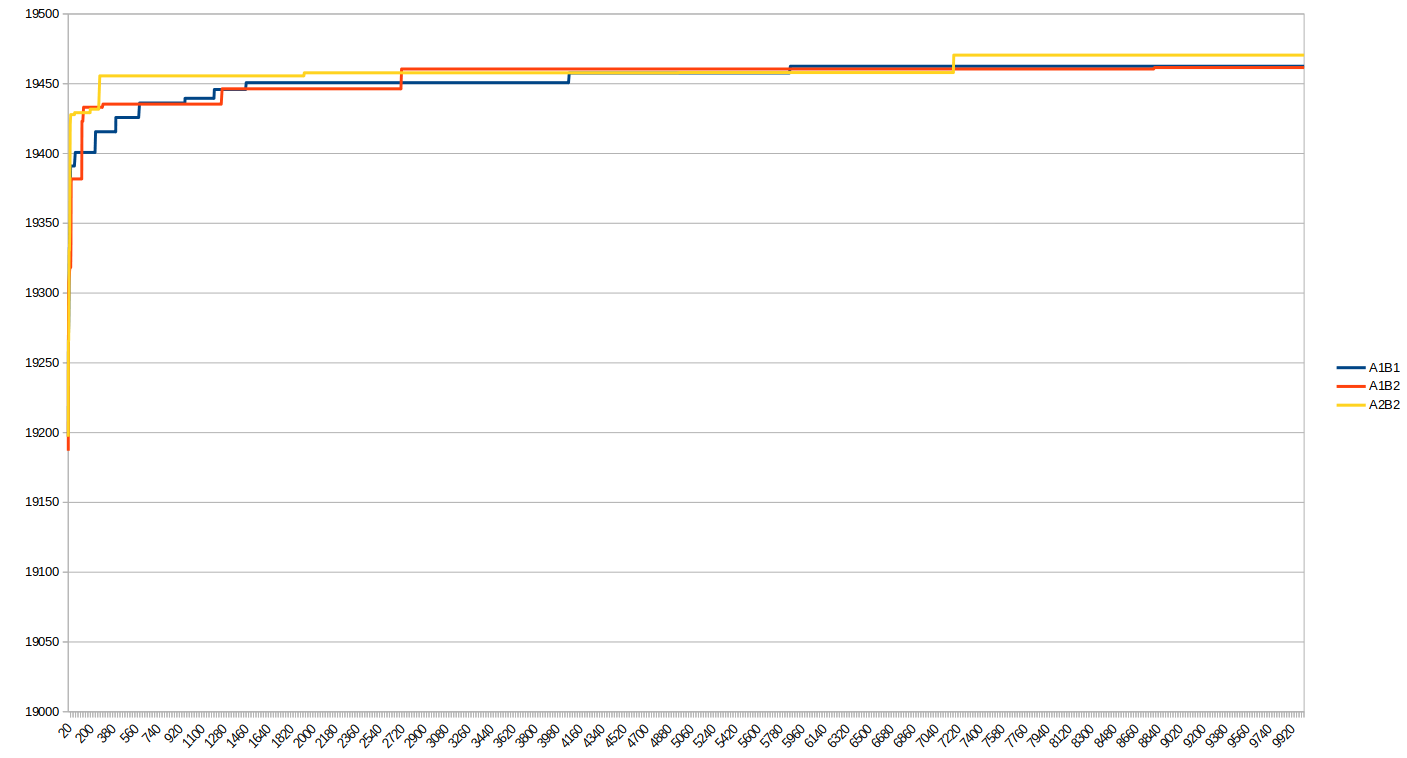
\includegraphics[scale=0.3]{img/GKD1conver.png}
		\caption{Evolución del mejor coste en la ejecución de todos los algoritmos respecto al número de evaluaciones para el problema GKD-c1, semilla 35608477}
		\label{gkd-c1_historico}
	\end{figure}

	\paragraph{}Para el problema GKD-c1 todas las configuraciones empiezan a encontrar soluciones aceptables desde la primera iteración realizada. Hemos considerado una solución aceptable aquella solución que difiere como máximo un 10\% respecto al óptimo global. En este problema las soluciones aceptables son todas aquellas cuyo coste es superior a 17.536,669.
	
	\paragraph{}En la ejecución de la configuración A1B1, el mejor coste obtenido se estabiliza en 19.462,505859375 a partir de las 5.844 iteraciones, permaneciendo inalterable hasta finalizar las 10.000 iteraciones objetivo. Esta configuración es capaz de encontrar costes con una diferencia inferior a un 1\% respecto al óptimo global a partir de las 10 iteraciones.
	
	\paragraph{}En la ejecución de la configuración A1B2, el mejor coste obtenido se estabiliza en 19.461,5625 a partir de las 8.791 iteraciones, permaneciendo inalterable hasta finalizar las 10.000 iteraciones objetivo. Esta configuración es capaz de encontrar costes con una diferencia inferior a un 1\% respecto al óptimo global a partir de las 3 iteraciones.
	
	\paragraph{}En la ejecución de la configuración A2B1, el mejor coste obtenido se estabiliza en 19.470,498046875 a partir de las 7.166 iteraciones, permaneciendo inalterable hasta finalizar las 10.000 iteraciones objetivo. Esta configuración es capaz de encontrar costes con una diferencia inferior a un 1\% respecto al óptimo global a partir de las 7 iteraciones.
	
	\paragraph{}En la configuración A1B1 obtenemos una diferencia entre el coste de la solución obtenida y el óptimo global de un 0.0011\% aproximadamente, siendo este último 19.485,188.
	
	\paragraph{}En la configuración A1B2 obtenemos una diferencia entre el coste de la solución obtenida y el óptimo global de un 0.0012\% aproximadamente.
	
	\paragraph{}En la configuración A2B1 obtenemos una diferencia entre el coste de la solución obtenida y el óptimo global de un 0.0007\% aproximadamente.	

	\begin{figure}[H]
		\centering
		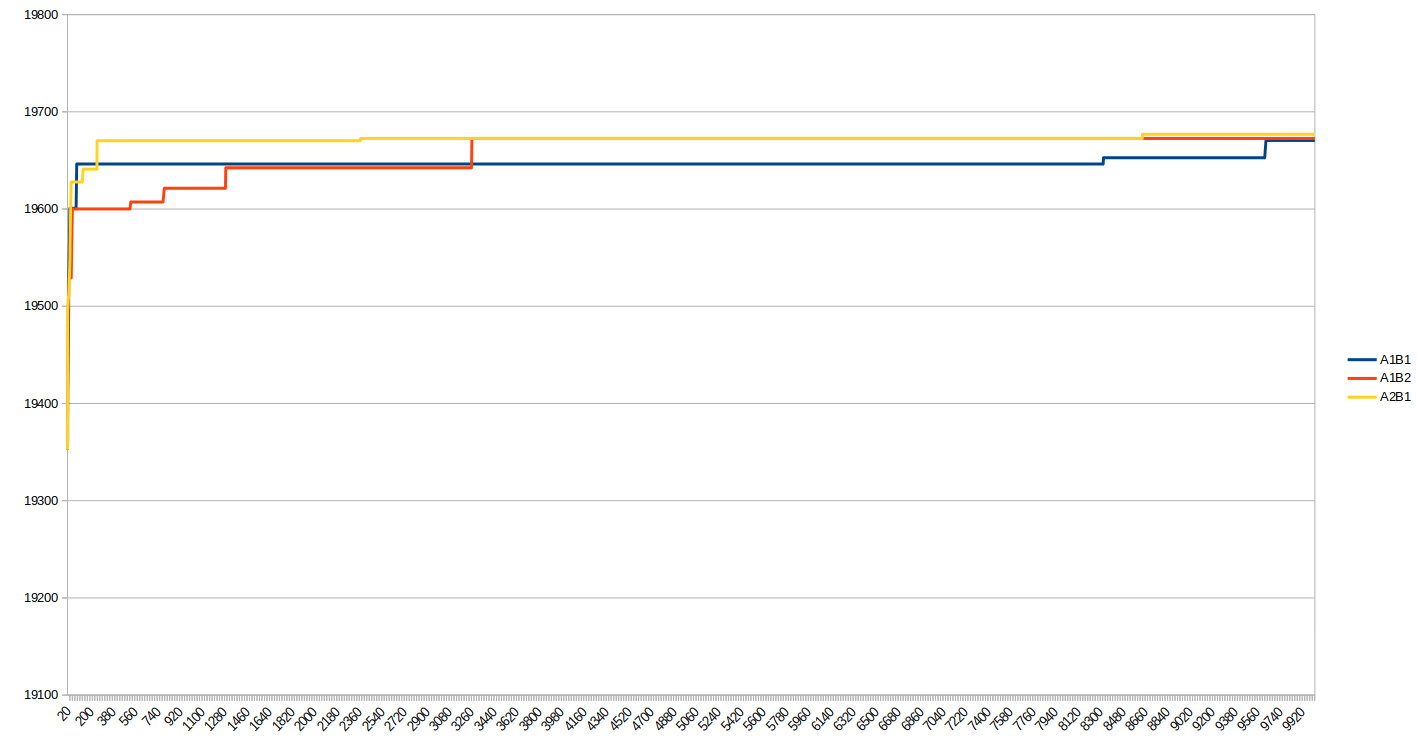
\includegraphics[scale=0.3]{img/GKD2conver.png}
		\caption{Evolución del mejor coste en la ejecución de todos los algoritmos 	respecto al número de evaluaciones para el problema GKD-c2, semilla 35608477}
		\label{gkd-c2_historico}
	\end{figure}

	\paragraph{}Para el problema GKD-c2 todas las configuraciones empiezan a encontrar soluciones aceptables desde la primera iteración realizada. Hemos considerado una solución aceptable aquella solución que difiere como máximo un 10\% respecto al óptimo global. En este problema las soluciones aceptables son todas aquellas cuyo coste es superior a 17.731,3833.
	
	\paragraph{}En la ejecución de la configuración A1B1, el mejor coste obtenido se estabiliza en 19.670,576171875 a partir de las 9.609 iteraciones, permaneciendo inalterable hasta finalizar las 10.000 iteraciones objetivo. Esta configuración es capaz de encontrar costes con una diferencia inferior a un 1\% respecto al óptimo global a partir de las 11 iteraciones.
	
	\paragraph{}En la ejecución de la configuración A1B2, el mejor coste obtenido se estabiliza en 19.672,58203125 a partir de las 3.243 iteraciones, permaneciendo inalterable hasta finalizar las 10.000 iteraciones objetivo. Esta configuración es capaz de encontrar costes con una diferencia inferior a un 1\% respecto al óptimo global a partir de las 11 iteraciones.
	
	\paragraph{}En la ejecución de la configuración A2B1, el mejor coste obtenido se estabiliza en 19.676,869140625 a partir de las 8.619 iteraciones, permaneciendo inalterable hasta finalizar las 10.000 iteraciones objetivo. Esta configuración es capaz de encontrar costes con una diferencia inferior a un 1\% respecto al óptimo global a partir de las 8 iteraciones.
	
	\paragraph{}En la configuración A1B1 obtenemos una diferencia entre el coste de la solución obtenida y el óptimo global de un 0.0015\% aproximadamente, siendo este último 19.701,537.
	
	\paragraph{}En la configuración A1B2 obtenemos una diferencia entre el coste de la solución obtenida y el óptimo global de un 0.0014\% aproximadamente.
	
	\paragraph{}En la configuración A2B1 obtenemos una diferencia entre el coste de la solución obtenida y el óptimo global de un 0.0012\% aproximadamente.

	\begin{figure}[H]
		\centering
		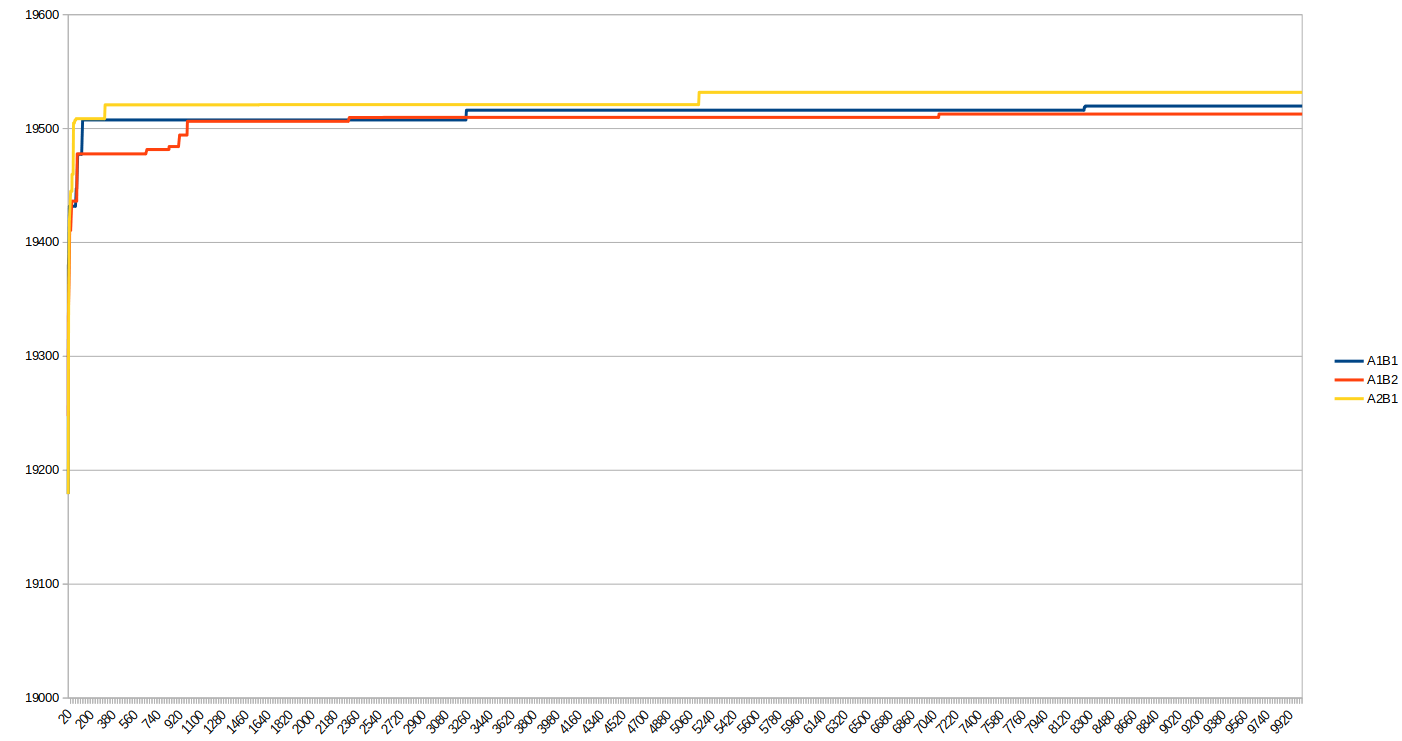
\includegraphics[scale=0.3]{img/GKD3conver.png}
		\caption{Evolución del mejor coste en la ejecución de todos los algoritmos respecto al número de evaluaciones para el problema GKD-c3, semilla 35608477}
		\label{gkd-c3_historico}
	\end{figure}

	\paragraph{}Para el problema GKD-c3 todas las configuraciones empiezan a encontrar soluciones aceptables desde la primera iteración realizada. Hemos considerado una solución aceptable aquella solución que difiere como máximo un 10\% respecto al óptimo global. En este problema las soluciones aceptables son todas aquellas cuyo coste es superior a 17.592,4863.
	
	\paragraph{}En la ejecución de la configuración A1B1, el mejor coste obtenido se estabiliza en 19.519,779296875 a partir de las 8.244 iteraciones, permaneciendo inalterable hasta finalizar las 10.000 iteraciones objetivo. Esta configuración es capaz de encontrar costes con una diferencia inferior a un 1\% respecto al óptimo global a partir de las 2 iteraciones.
	
	\paragraph{}En la ejecución de la configuración A1B2, el mejor coste obtenido se estabiliza en 19.512,7109375 a partir de las 7.058 iteraciones, permaneciendo inalterable hasta finalizar las 10.000 iteraciones objetivo. Esta configuración es capaz de encontrar costes con una diferencia inferior a un 1\% respecto al óptimo global a partir de las 9 iteraciones.
	
	\paragraph{}En la ejecución de la configuración A2B1, el mejor coste obtenido se estabiliza en 19.531,783203125 a partir de las 5.114 iteraciones, permaneciendo inalterable hasta finalizar las 10.000 iteraciones objetivo. Esta configuración es capaz de encontrar costes con una diferencia inferior a un 1\% respecto al óptimo global a partir de las 5 iteraciones.
	
	\paragraph{}En la configuración A1B1 obtenemos una diferencia entre el coste de la solución obtenida y el óptimo global de un 0.0014\% aproximadamente, siendo este último 19.547,207.
	
	\paragraph{}En la configuración A1B2 obtenemos una diferencia entre el coste de la solución obtenida y el óptimo global de un 0.0017\% aproximadamente.
	
	\paragraph{}En la configuración A2B1 obtenemos una diferencia entre el coste de la solución obtenida y el óptimo global de un 0.0007\% aproximadamente.

	\begin{figure}[H]
		\centering
		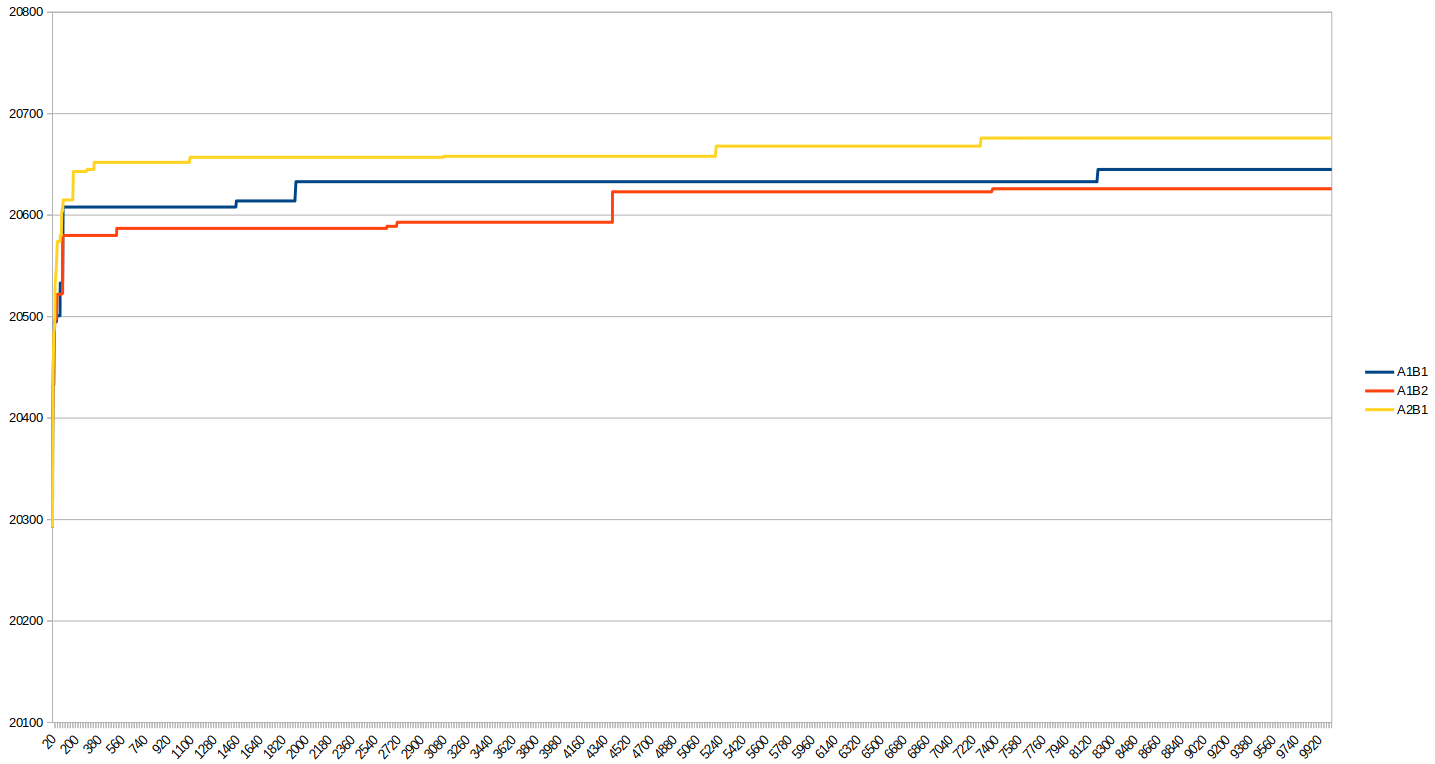
\includegraphics[scale=0.3]{img/SOM1conver.png}
		\caption{Evolución del mejor coste en la ejecución de todos los algoritmos respecto al número de evaluaciones para el problema SOM-b11, semilla 35608477}
		\label{SOM-b_11_historico}
	\end{figure}

	\paragraph{}Para el problema SOM-b11 todas las configuraciones empiezan a encontrar soluciones aceptables desde la primera iteración realizada. Hemos considerado una solución aceptable aquella solución que difiere como máximo un 10\% respecto al óptimo global. En este problema las soluciones aceptables son todas aquellas cuyo coste es superior a 18.668,7.
	
	\paragraph{}En la ejecución de la configuración A1B1, el mejor coste obtenido se estabiliza en 20.645 a partir de las 8.174 iteraciones, permaneciendo inalterable hasta finalizar las 10.000 iteraciones objetivo. Esta configuración es capaz de encontrar costes con una diferencia inferior a un 1\% respecto al óptimo global a partir de las 84 iteraciones.
	
	\paragraph{}En la ejecución de la configuración A1B2, el mejor coste obtenido se estabiliza en 20.626 a partir de las 7.351 iteraciones, permaneciendo inalterable hasta finalizar las 10.000 iteraciones objetivo. Esta configuración es capaz de encontrar costes con una diferencia inferior a un 1\% respecto al óptimo global a partir de las 82 iteraciones.
	
	\paragraph{}En la ejecución de la configuración A2B1, el mejor coste obtenido se estabiliza en 20.676 a partir de las 7.260 iteraciones, permaneciendo inalterable hasta finalizar las 10.000 iteraciones objetivo. Esta configuración es capaz de encontrar costes con una diferencia inferior a un 1\% respecto al óptimo global a partir de las 31 iteraciones.
	
	\paragraph{}En la configuración A1B1 obtenemos una diferencia entre el coste de la solución obtenida y el óptimo global de un 0.0047\% aproximadamente, siendo este último 20.743.
	
	\paragraph{}En la configuración A1B2 obtenemos una diferencia entre el coste de la solución obtenida y el óptimo global de un 0.0056\% aproximadamente.
	
	\paragraph{}En la configuración A2B1 obtenemos una diferencia entre el coste de la solución obtenida y el óptimo global de un 0.0032\% aproximadamente.

	\begin{figure}[H]
		\centering
		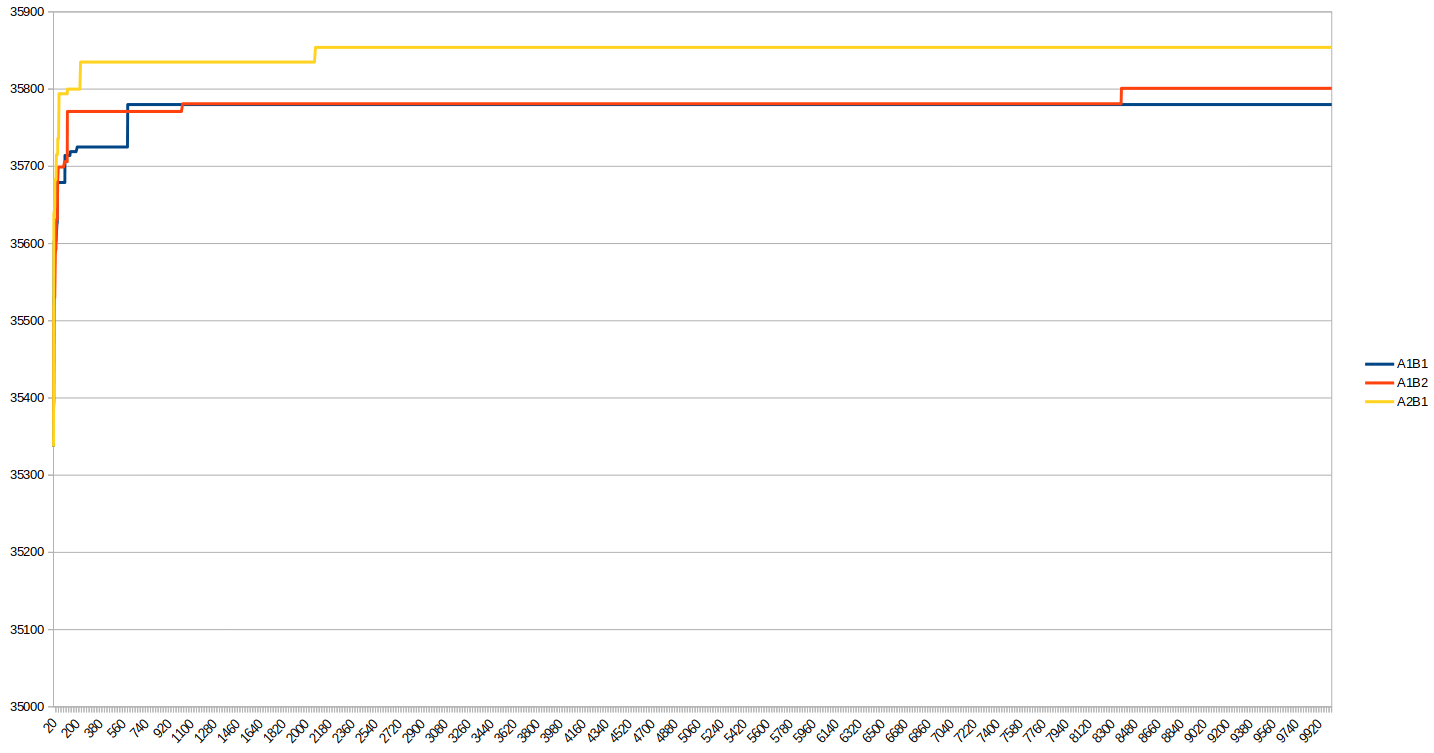
\includegraphics[scale=0.3]{img/SOM2conver.png}
		\caption{Evolución del mejor coste en la ejecución de todos los algoritmos respecto al número de evaluaciones para el problema SOM-b12, semilla 35608477}
		\label{SOM-b_12_historico}
	\end{figure}

	\paragraph{}Para el problema SOM-b12 todas las configuraciones empiezan a encontrar soluciones aceptables desde la primera iteración realizada. Hemos considerado una solución aceptable aquella solución que difiere como máximo un 10\% respecto al óptimo global. En este problema las soluciones aceptables son todas aquellas cuyo coste es superior a 32.292,9.
	
	\paragraph{}En la ejecución de la configuración A1B1, el mejor coste obtenido se estabiliza en 35.780 a partir de las 582 iteraciones, permaneciendo inalterable hasta finalizar las 10.000 iteraciones objetivo. Esta configuración es capaz de encontrar costes con una diferencia inferior a un 1\% respecto al óptimo global a partir de las 6 iteraciones.
	
	\paragraph{}En la ejecución de la configuración A1B2, el mejor coste obtenido se estabiliza en 35.801 a partir de las 8.356 iteraciones, permaneciendo inalterable hasta finalizar las 10.000 iteraciones objetivo. Esta configuración es capaz de encontrar costes con una diferencia inferior a un 1\% respecto al óptimo global a partir de las 7 iteraciones.
	
	\paragraph{}En la ejecución de la configuración A2B1, el mejor coste obtenido se estabiliza en 35.854 a partir de las 2.051 iteraciones, permaneciendo inalterable hasta finalizar las 10.000 iteraciones objetivo. Esta configuración es capaz de encontrar costes con una diferencia inferior a un 1\% respecto al óptimo global a partir de las 4 iteraciones.
	
	\paragraph{}En la configuración A1B1 obtenemos una diferencia entre el coste de la solución obtenida y el óptimo global de un 0.0028\% aproximadamente, siendo este último 35.881.
	
	\paragraph{}En la configuración A1B2 obtenemos una diferencia entre el coste de la solución obtenida y el óptimo global de un 0.0022\% aproximadamente.
	
	\paragraph{}En la configuración A2B1 obtenemos una diferencia entre el coste de la solución obtenida y el óptimo global de un 0.0007\% aproximadamente.

	\begin{figure}[H]
		\centering
		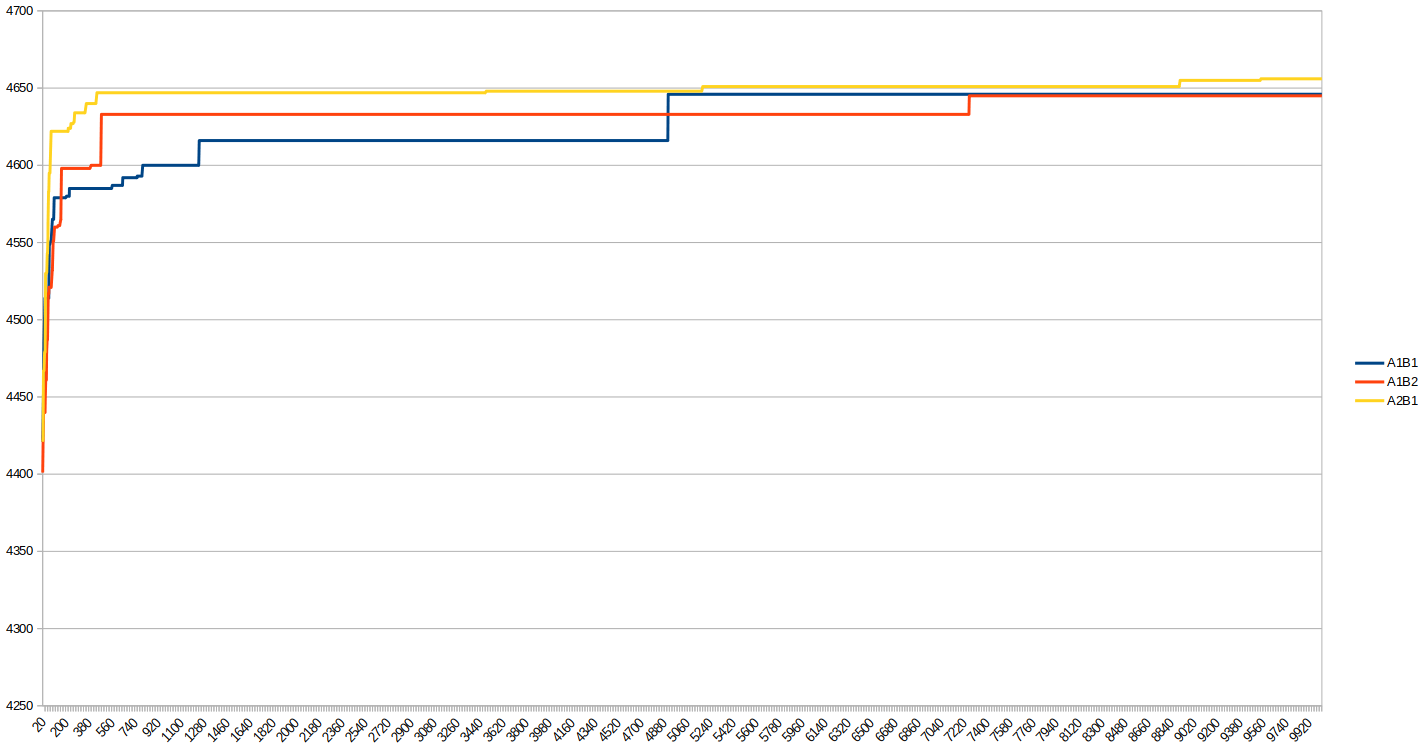
\includegraphics[scale=0.3]{img/SOM3conver.png}
		\caption{Evolución del mejor coste en la ejecución de todos los algoritmos respecto al número de evaluaciones para el problema SOM-b13, semilla 35608477}
		\label{SOM-b_13_historico}
	\end{figure}

	\paragraph{}Para el problema SOM-b13 todas las configuraciones empiezan a encontrar soluciones aceptables desde la primera iteración realizada. Hemos considerado una solución aceptable aquella solución que difiere como máximo un 10\% respecto al óptimo global. En este problema las soluciones aceptables son todas aquellas cuyo coste es superior a 4.192,2.
	
	\paragraph{}En la ejecución de la configuración A1B1, el mejor coste obtenido se estabiliza en 4.646 a partir de las 4.891 iteraciones, permaneciendo inalterable hasta finalizar las 10.000 iteraciones objetivo. Esta configuración es capaz de encontrar costes con una diferencia inferior a un 1\% respecto al óptimo global a partir de las 1.225 iteraciones.
	
	\paragraph{}En la ejecución de la configuración A1B2, el mejor coste obtenido se estabiliza en 4.645 a partir de las 7.245 iteraciones, permaneciendo inalterable hasta finalizar las 10.000 iteraciones objetivo. Esta configuración es capaz de encontrar costes con una diferencia inferior a un 1\% respecto al óptimo global a partir de las 460 iteraciones.
	
	\paragraph{}En la ejecución de la configuración A2B1, el mejor coste obtenido se estabiliza en 4.656 a partir de las 9.525 iteraciones, permaneciendo inalterable hasta finalizar las 10.000 iteraciones objetivo. Esta configuración es capaz de encontrar costes con una diferencia inferior a un 1\% respecto al óptimo global a partir de las 67 iteraciones.
	
	\paragraph{}En la configuración A1B1 obtenemos una diferencia entre el coste de la solución obtenida y el óptimo global de un 0.0025\% aproximadamente, siendo este último 4.658.
	
	\paragraph{}En la configuración A1B2 obtenemos una diferencia entre el coste de la solución obtenida y el óptimo global de un 0.0027\% aproximadamente.
	
	\paragraph{}En la configuración A2B1 obtenemos una diferencia entre el coste de la solución obtenida y el óptimo global de un 0.0004\% aproximadamente.

	\begin{figure}[H]
		\centering
		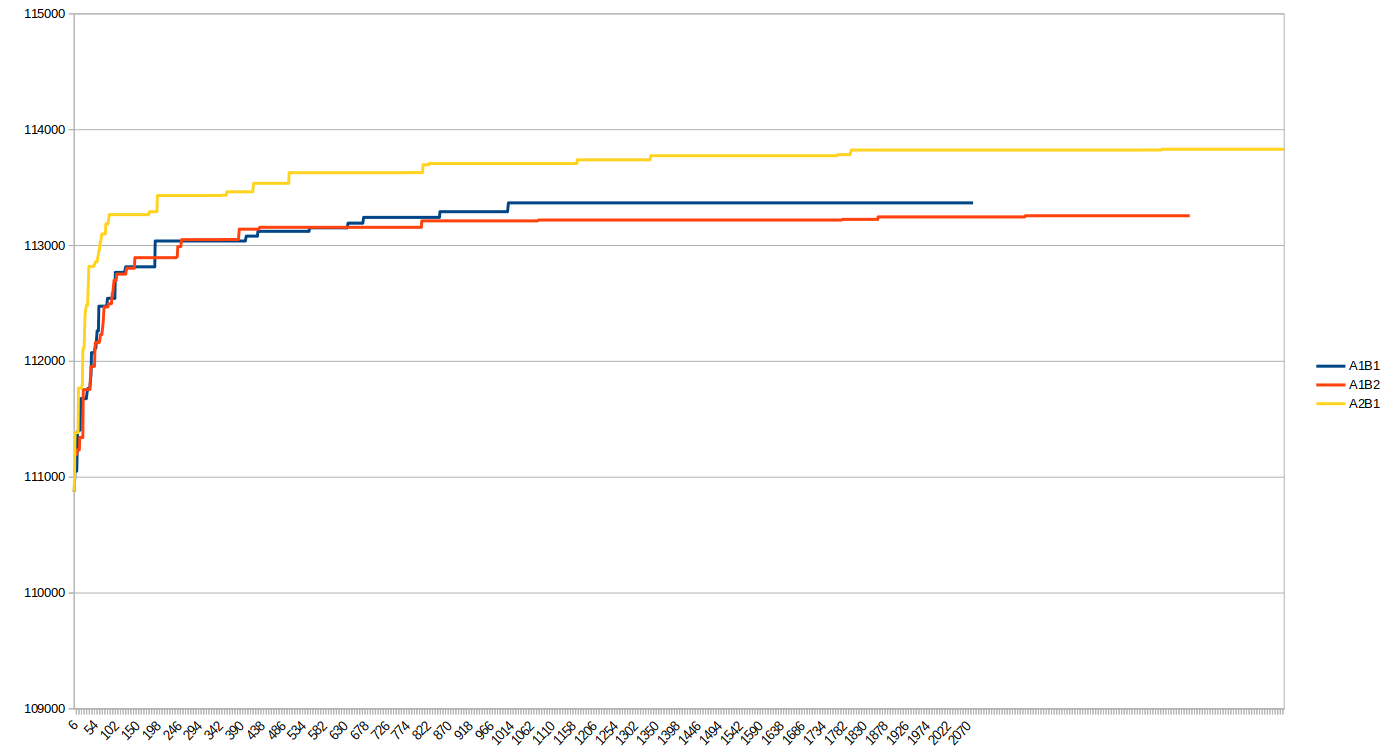
\includegraphics[scale=0.3]{img/MDG1conver.png}
		\caption{Evolución del mejor coste en la ejecución de todos los algoritmos respecto al número de evaluaciones para el problema MDG-a21, semilla 35608477}
		\label{MDG-a_21_historico}
	\end{figure}

	\paragraph{}Para el problema MDG-a21 todas las configuraciones empiezan a encontrar soluciones aceptables desde la primera iteración realizada. Hemos considerado una solución aceptable aquella solución que difiere como máximo un 10\% respecto al óptimo global. En este problema las soluciones aceptables son todas aquellas cuyo coste es superior a 102.833,1.
	
	\paragraph{}En la ejecución de la configuración A1B1, el mejor coste obtenido se estabiliza en 113.368 a partir de las 1.003 iteraciones, permaneciendo inalterable hasta realizar 2.076 iteraciones, donde se termina la ejecución al haber alcanzado los 600 segundos límites de tiempo de ejecución. Esta configuración es capaz de encontrar costes con una diferencia inferior a un 1\% respecto al óptimo global a partir de las 425 iteraciones.
	
	\paragraph{}En la ejecución de la configuración A1B2, el mejor coste obtenido se estabiliza en 113.257 a partir de las 2.196 iteraciones, permaneciendo inalterable hasta realizar 2.575 iteraciones, donde se termina la ejecución al haber alcanzado los 600 segundos límites de tiempo de ejecución. Esta configuración es capaz de encontrar costes con una diferencia inferior a un 1\% respecto al óptimo global a partir de las 382 iteraciones.
	
	\paragraph{}En la ejecución de la configuración A2B1, el mejor coste obtenido se estabiliza en 113.831 a partir de las 2.511 iteraciones, permaneciendo inalterable hasta realizar 2.793 iteraciones, donde se termina la ejecución al haber alcanzado los 600 segundos límites de tiempo de ejecución. Esta configuración es capaz de encontrar costes con una diferencia inferior a un 1\% respecto al óptimo global a partir de las 74 iteraciones.
	
	\paragraph{}En la configuración A1B1 obtenemos una diferencia entre el coste de la solución obtenida y el óptimo global de un 0.0077\% aproximadamente, siendo este último 114.259.
	
	\paragraph{}En la configuración A1B2 obtenemos una diferencia entre el coste de la solución obtenida y el óptimo global de un 0.0087\% aproximadamente.
	
	\paragraph{}En la configuración A2B1 obtenemos una diferencia entre el coste de la solución obtenida y el óptimo global de un 0.0037\% aproximadamente.

	\begin{figure}[H]
		\centering
		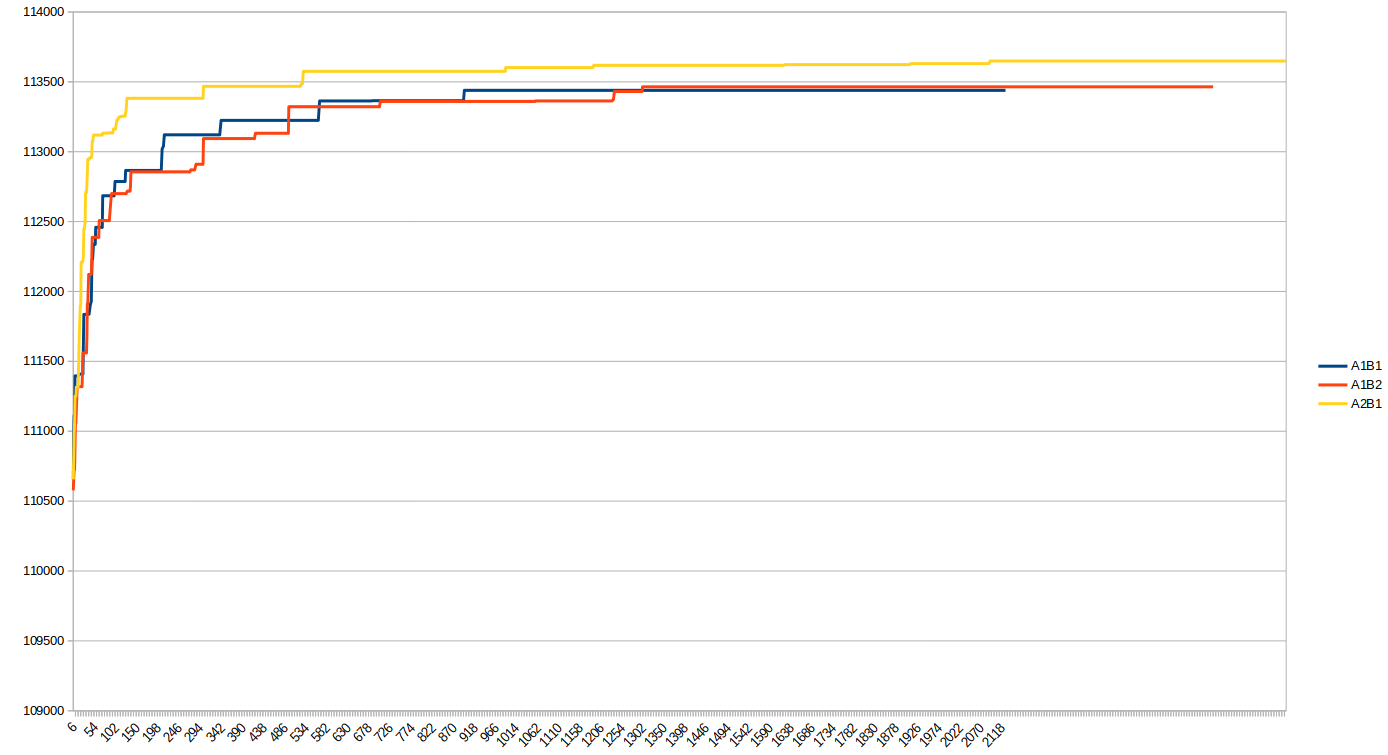
\includegraphics[scale=0.3]{img/MDG2conver.png}
		\caption{Evolución del mejor coste en la ejecución de todos los algoritmos respecto al número de evaluaciones para el problema MDG-a22, semilla 35608477}
		\label{MDG-a_22_historico}
	\end{figure}

	\paragraph{}Para el problema MDG-a22 todas las configuraciones empiezan a encontrar soluciones aceptables desde la primera iteración realizada. Hemos considerado una solución aceptable aquella solución que difiere como máximo un 10\% respecto al óptimo global. En este problema las soluciones aceptables son todas aquellas cuyo coste es superior a 102.894,3.
	
	\paragraph{}En la ejecución de la configuración A1B1, el mejor coste obtenido se estabiliza en 113.439 a partir de las 890 iteraciones, permaneciendo inalterable hasta realizar 2.121 iteraciones, donde se termina la ejecución al haber alcanzado los 600 segundos límites de tiempo de ejecución. Esta configuración es capaz de encontrar costes con una diferencia inferior a un 1\% respecto al óptimo global a partir de las 337 iteraciones.
	
	\paragraph{}En la ejecución de la configuración A1B2, el mejor coste obtenido se estabiliza en 113.464 a partir de las 1.295 iteraciones, permaneciendo inalterable hasta realizar 2.592 iteraciones, donde se termina la ejecución al haber alcanzado los 600 segundos límites de tiempo de ejecución. Esta configuración es capaz de encontrar costes con una diferencia inferior a un 1\% respecto al óptimo global a partir de las 491 iteraciones.
	
	\paragraph{}En la ejecución de la configuración A2B1, el mejor coste obtenido se estabiliza en 113.649 a partir de las 2.085 iteraciones, permaneciendo inalterable hasta realizar 2.758 iteraciones, donde se termina la ejecución al haber alcanzado los 600 segundos límites de tiempo de ejecución. Esta configuración es capaz de encontrar costes con una diferencia inferior a un 1\% respecto al óptimo global a partir de las 100 iteraciones.
	
	\paragraph{}En la configuración A1B1 obtenemos una diferencia entre el coste de la solución obtenida y el óptimo global de un 0.0077\% aproximadamente, siendo este último 114.327.
	
	\paragraph{}En la configuración A1B2 obtenemos una diferencia entre el coste de la solución obtenida y el óptimo global de un 0.0075\% aproximadamente.
	
	\paragraph{}En la configuración A2B1 obtenemos una diferencia entre el coste de la solución obtenida y el óptimo global de un 0.0059\% aproximadamente.

	\begin{figure}[H]
		\centering
		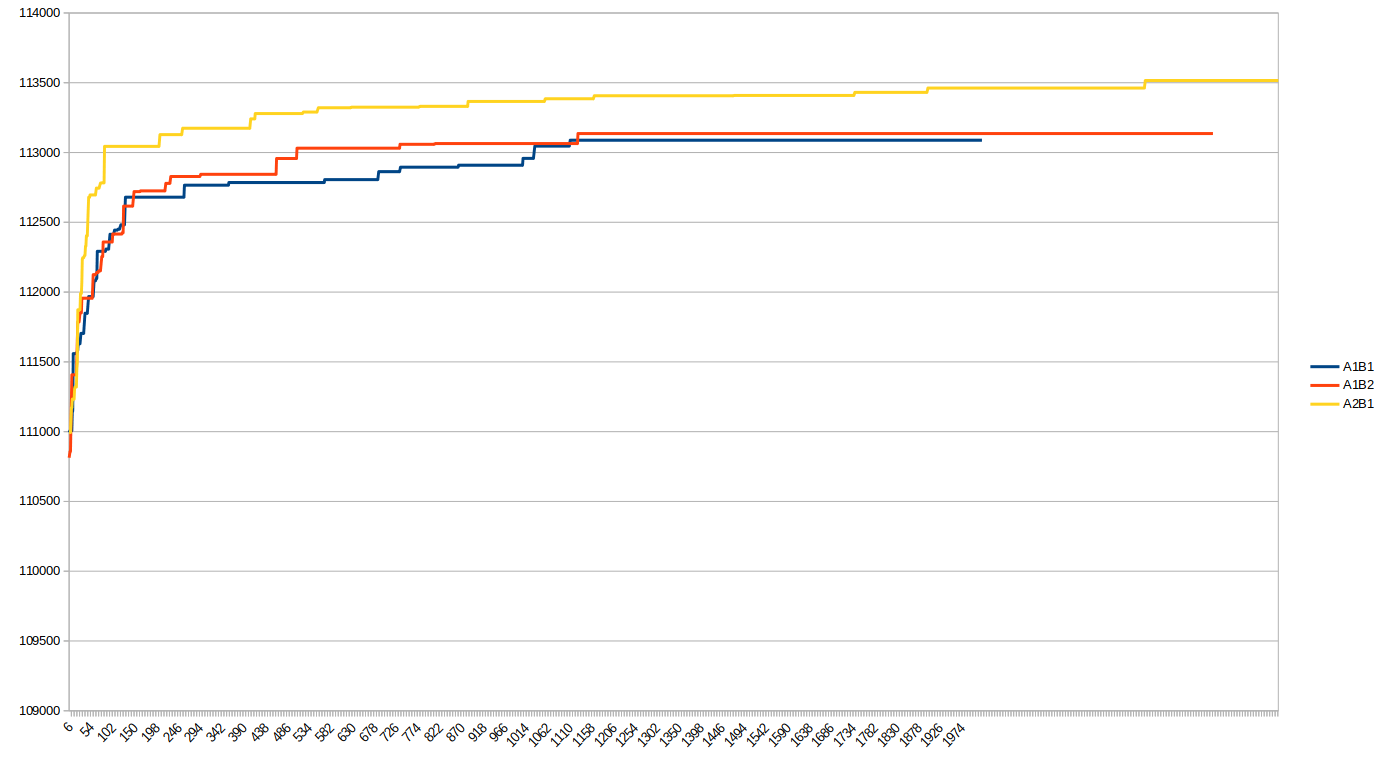
\includegraphics[scale=0.3]{img/MDG3conver.png}
		\caption{Evolución del mejor coste en la ejecución de todos los algoritmos respecto al número de evaluaciones para el problema MDG-a23, semilla 35608477}
		\label{MDG-a_23_historico}
	\end{figure}

	\paragraph{}Para el problema MDG-a23 todas las configuraciones empiezan a encontrar soluciones aceptables desde la primera iteración realizada. Hemos considerado una solución aceptable aquella solución que difiere como máximo un 10\% respecto al óptimo global. En este problema las soluciones aceptables son todas aquellas cuyo coste es superior a 102.710,7.
	
	\paragraph{}En la ejecución de la configuración A1B1, el mejor coste obtenido se estabiliza en 113.088 a partir de las 1.105 iteraciones, permaneciendo inalterable hasta realizar 2.012 iteraciones, donde se termina la ejecución al haber alcanzado los 600 segundos límites de tiempo de ejecución. Esta configuración es capaz de encontrar costes con una diferencia inferior a un 1\% respecto al óptimo global a partir de las 1.027 iteraciones.
	
	\paragraph{}En la ejecución de la configuración A1B2, el mejor coste obtenido se estabiliza en 113.136 a partir de las 1.122 iteraciones, permaneciendo inalterable hasta realizar 2.521 iteraciones, donde se termina la ejecución al haber alcanzado los 600 segundos límites de tiempo de ejecución. Esta configuración es capaz de encontrar costes con una diferencia inferior a un 1\% respecto al óptimo global a partir de las 503 iteraciones.
	
	\paragraph{}En la ejecución de la configuración A2B1, el mejor coste obtenido se estabiliza en 113.516 a partir de las 2.372 iteraciones, permaneciendo inalterable hasta realizar 2.665 iteraciones, donde se termina la ejecución al haber alcanzado los 600 segundos límites de tiempo de ejecución. Esta configuración es capaz de encontrar costes con una diferencia inferior a un 1\% respecto al óptimo global a partir de las 79 iteraciones.
	
	\paragraph{}En la configuración A1B1 obtenemos una diferencia entre el coste de la solución obtenida y el óptimo global de un 0.0090\% aproximadamente, siendo este último 114.123.
	
	\paragraph{}En la configuración A1B2 obtenemos una diferencia entre el coste de la solución obtenida y el óptimo global de un 0.0086\% aproximadamente.
	
	\paragraph{}En la configuración A2B1 obtenemos una diferencia entre el coste de la solución obtenida y el óptimo global de un 0.0053\% aproximadamente.
	
	\subsection{$\alpha$ = 1, $\beta$ =1 vs $\alpha$ = 1, $\beta$ =2 vs $\alpha$ = 2, $\beta$ =1}
	
	\paragraph{}A continuación, se muestran los gráficos de cajas y bigotes para cada problema de la serie GKD (Figura 11, 12 y 13). En ellos se pueden comparar a simple vista tanto los resultados obtenidos como la agrupación de los mismos.
	
	\begin{figure}[H]
		\centering
		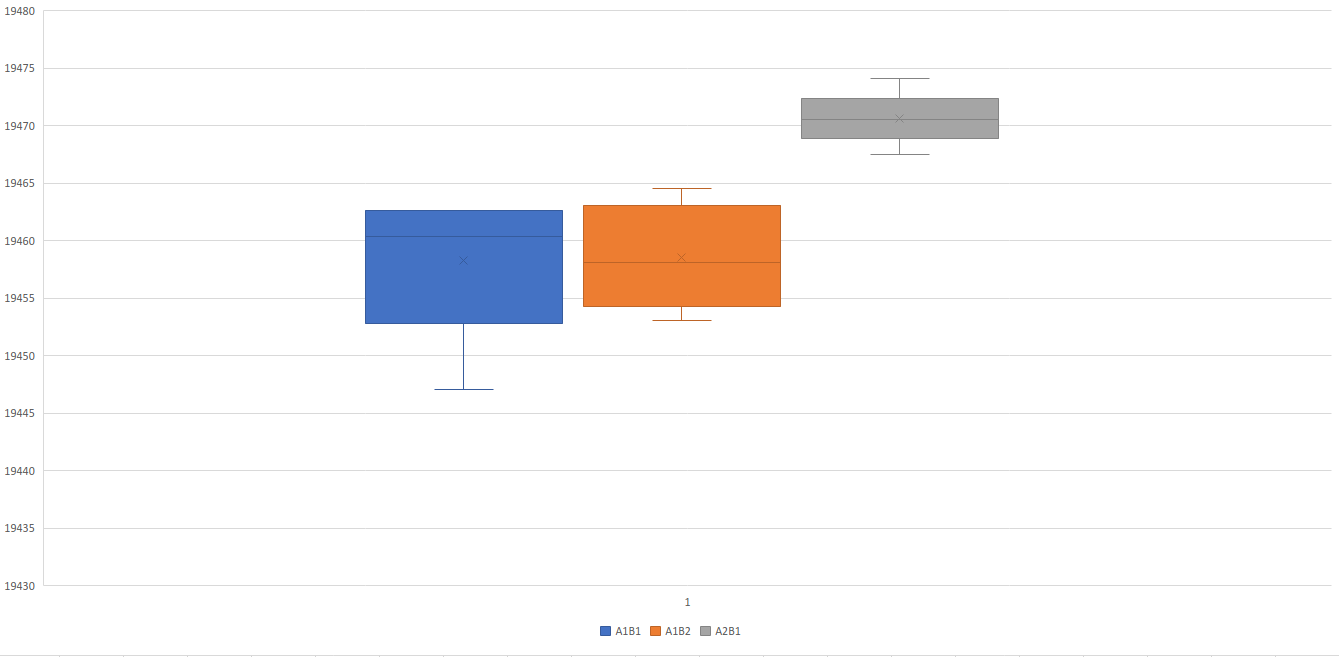
\includegraphics[scale=0.3]{img/BIGOTESGKD1.png}
		\caption{Gráfica de cajas y bigotes para el problema GKD-c1}
		\label{gkd-c1_bigotes}
	\end{figure}

	\paragraph{}Para el problema GKD-c1, los resultados obtenidos para las configuraciones A1B1 y A1B2 son muy similares, obteniendo ligeramente un mayor agrupamiento el algoritmo con la configuración A1B2. Se puede observar como la configuración A2B1 obtiene mejores resultados y agrupamiento de los mismos.

	\begin{figure}[H]
		\centering
		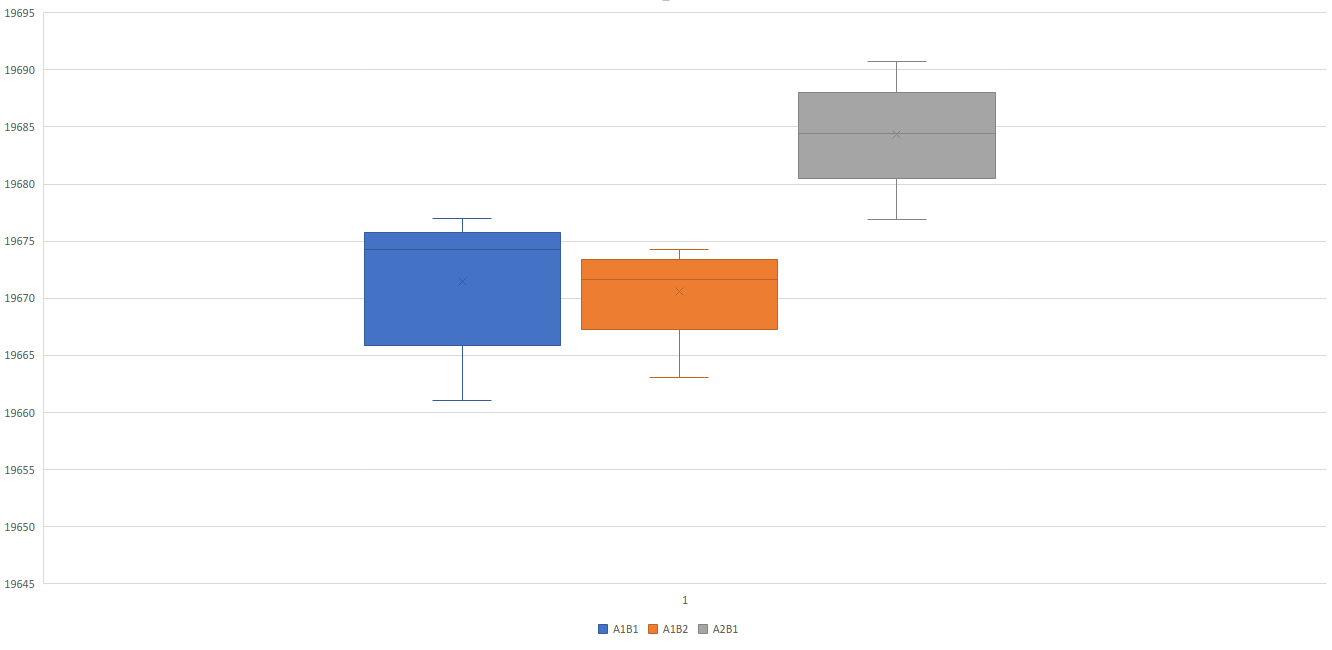
\includegraphics[scale=0.3]{img/BIGOTESGKD2.png}
		\caption{Gráfica de cajas y bigotes para el problema GKD-c2}
		\label{gkd-c2_bigotes}
	\end{figure}

	\begin{figure}[H]
		\centering
		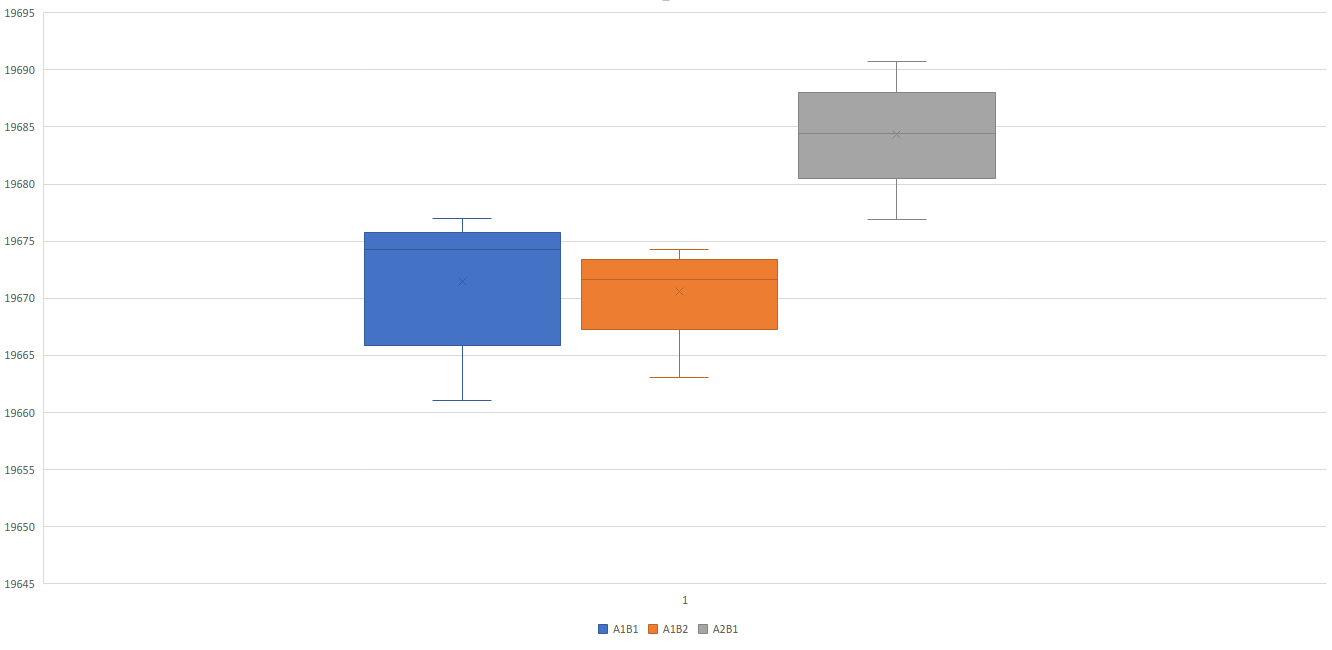
\includegraphics[scale=0.3]{img/BIGOTESGKD2.png}
		\caption{Gráfica de cajas y bigotes para el problema GKD-c3}
		\label{gkd-c3_bigotes}
	\end{figure}

	\paragraph{}Para los problemas GKD-c2 y GKD-c3, la configuración que obtiene un mejor agrupamiento de los resultados obtenidos es A1B2, seguida de A2B1, siendo A1B1 la que obtiene un peor agrupamiento. En cuanto a resultados obtenidos, las configuraciones A1B1 y A1B2 obtienen unas soluciones bastante similares, siendo la configuración A2B1 la mejor de todas.
	
	\paragraph{}Ahora, se analizarán los gráficos de cajas y bigotes correspondientes con las serie de datos SOM (Figura 14, 15 y 16).
	
	\begin{figure}[H]
		\centering
		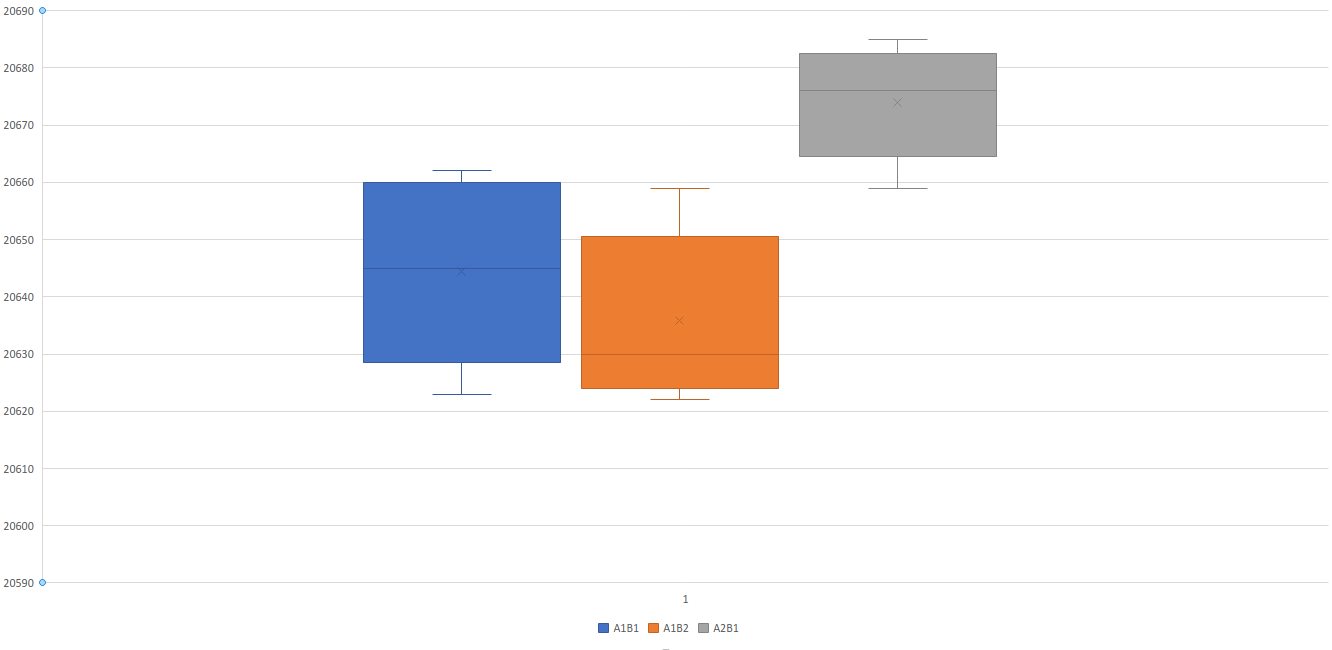
\includegraphics[scale=0.3]{img/BIGOTESSOM1.png}
		\caption{Gráfica de cajas y bigotes para el problema SOM-b11}
		\label{SOM-b11_bigotes}
	\end{figure}

	\begin{figure}[H]
		\centering
		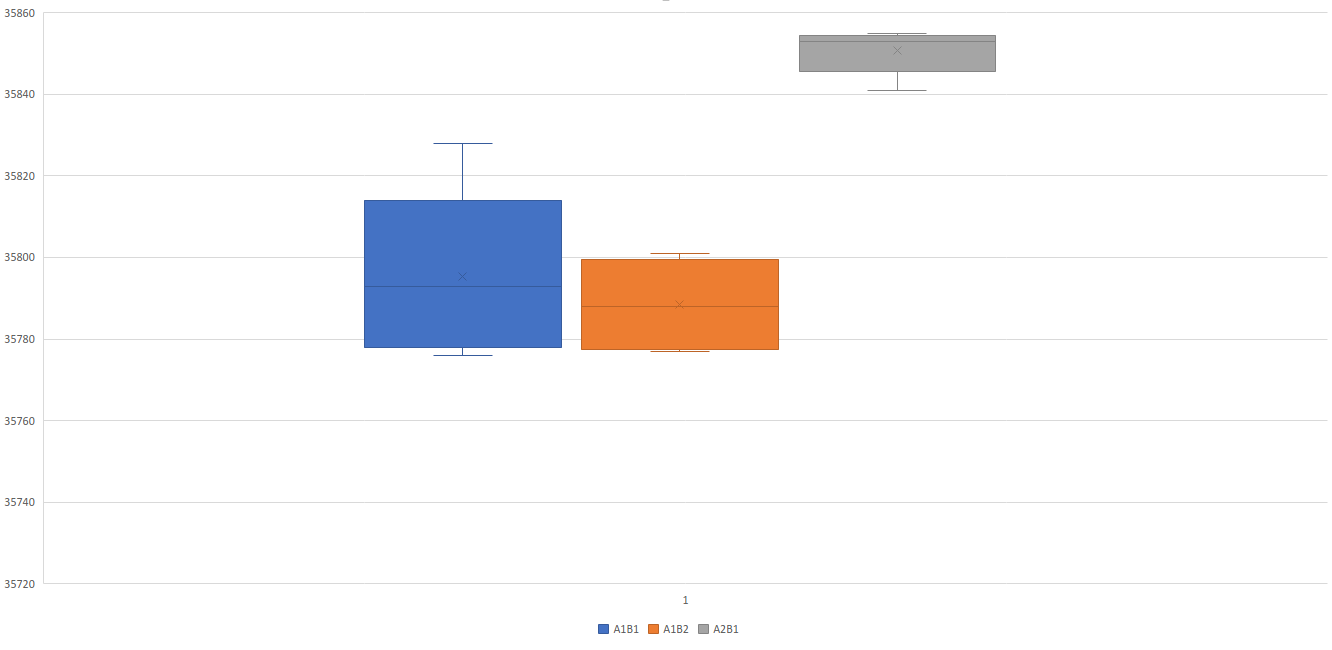
\includegraphics[scale=0.3]{img/BIGOTESSOM2.png}
		\caption{Gráfica de cajas y bigotes para el problema SOM-b12}
		\label{SOM-b12_bigotes}
	\end{figure}

	\paragraph{}Para los problemas SOM-b11 y SOM-b12, en cuanto a agrupamiento de los resultados, la configuración A2B1 es la mejor, seguida de A1B2 y A1B1. En cuanto a mejores resultados obtenidos, la configuración A2B1 es también la mejor, seguida de A1B2 y A1B1. En el problema SOM-b12, cabe destacar la robustez de la configuración A2B1. 

	\begin{figure}[H]
		\centering
		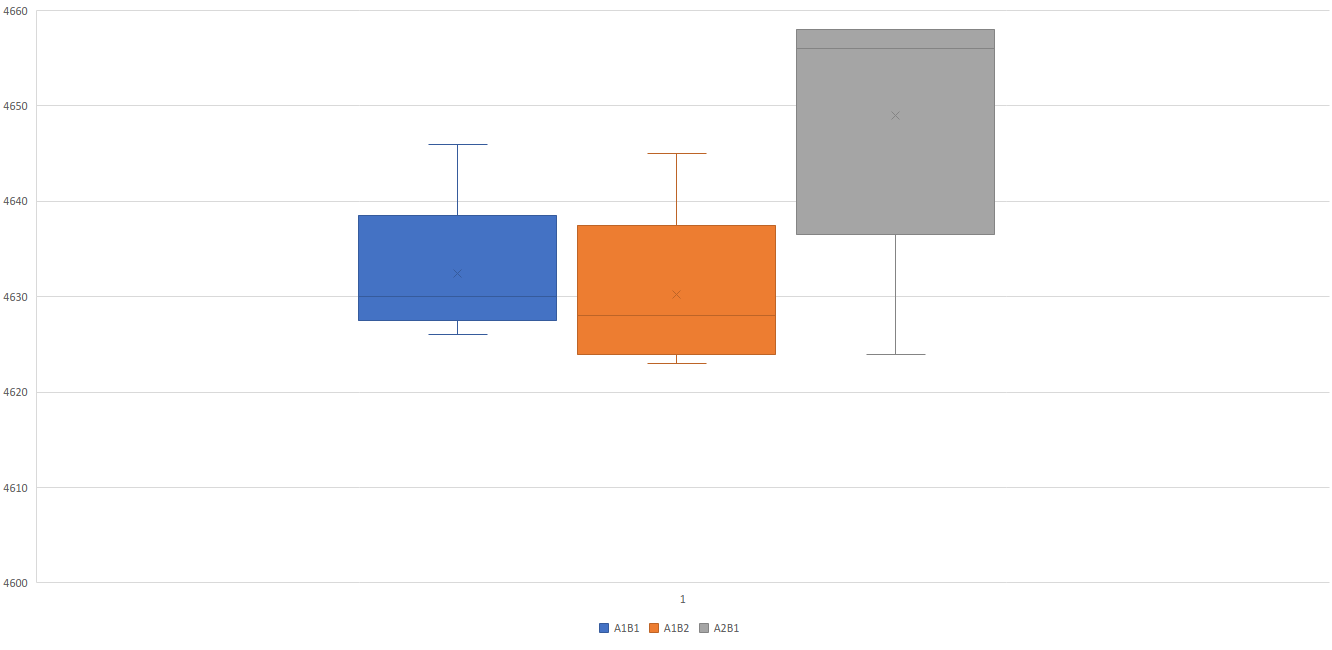
\includegraphics[scale=0.3]{img/BIGOTESSOM3.png}
		\caption{Gráfica de cajas y bigotes para el problema SOM-b13}
		\label{SOM-b13_bigotes}
	\end{figure}

	\paragraph{}En el problema SOM-b13, a diferencia de los anteriores casos, la configuración A2B1 obtiene el peor agrupamiento de resultados, siendo la mejor configuración A1B1, seguida de A1B2. En cuanto a calidad de soluciones, la configuración A2B1 es la mejor, seguida de A1B1 y de A1B2 en último lugar.
	
	\paragraph{}Los tres últimos gráficos de cajas y bigotes se corresponden con las serie de datos MDG (Figura 17, 18 y 19). A continuación, pasamos a analizarlas.

	\begin{figure}[H]
		\centering
		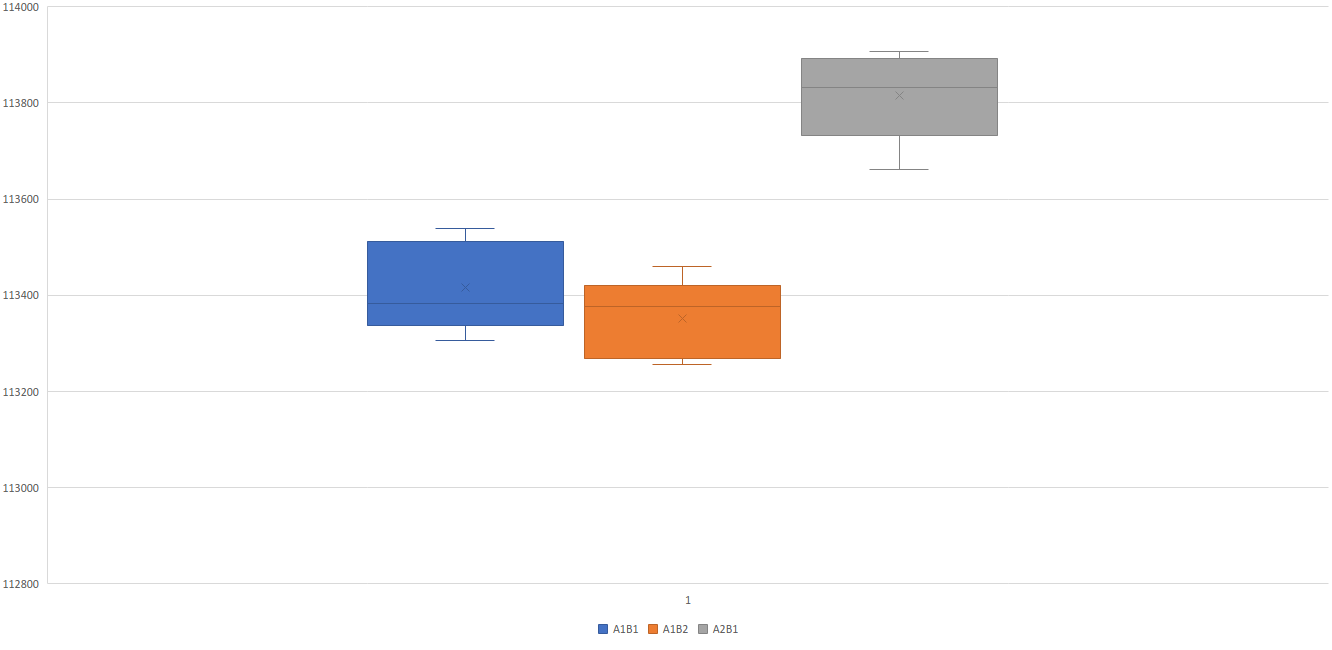
\includegraphics[scale=0.3]{img/BIGOTESMDG1.png}
		\caption{Gráfica de cajas y bigotes para el problema MDG-a21}
		\label{MDG-a21_bigotes}
	\end{figure}

	\paragraph{}En el problema MDG-a21 las agrupaciones de los resultados de las tres configuraciones del S.C.H. son prácticamente similares. No obstante, en cuanto a resultados, la configuración A2B1 es la que mejor rendimiento obtiene, seguida de A1B1 y A1B2 en último lugar.

	\begin{figure}[H]
		\centering
		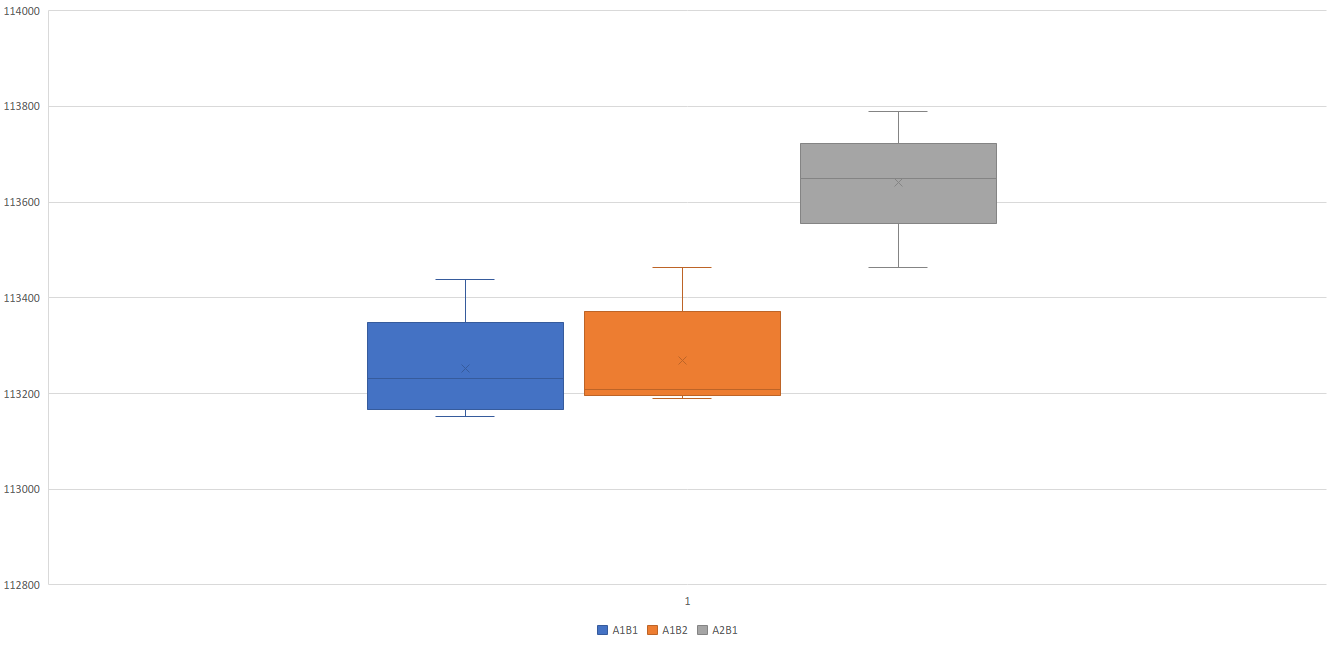
\includegraphics[scale=0.3]{img/BIGOTESMDG2.png}
		\caption{Gráfica de cajas y bigotes para el problema MDG-a22}
		\label{MDG-a22_bigotes}
	\end{figure}

	\paragraph{}En el problema MDG-a22, al igual que en MDG-a21, el agrupamiento de las soluciones obtenidas para las tres configuraciones son similares. En cuanto a resultados obtenidos, la mejor configuración es A2B1, seguida de A1B2 y A1B1.

	\begin{figure}[H]
		\centering
		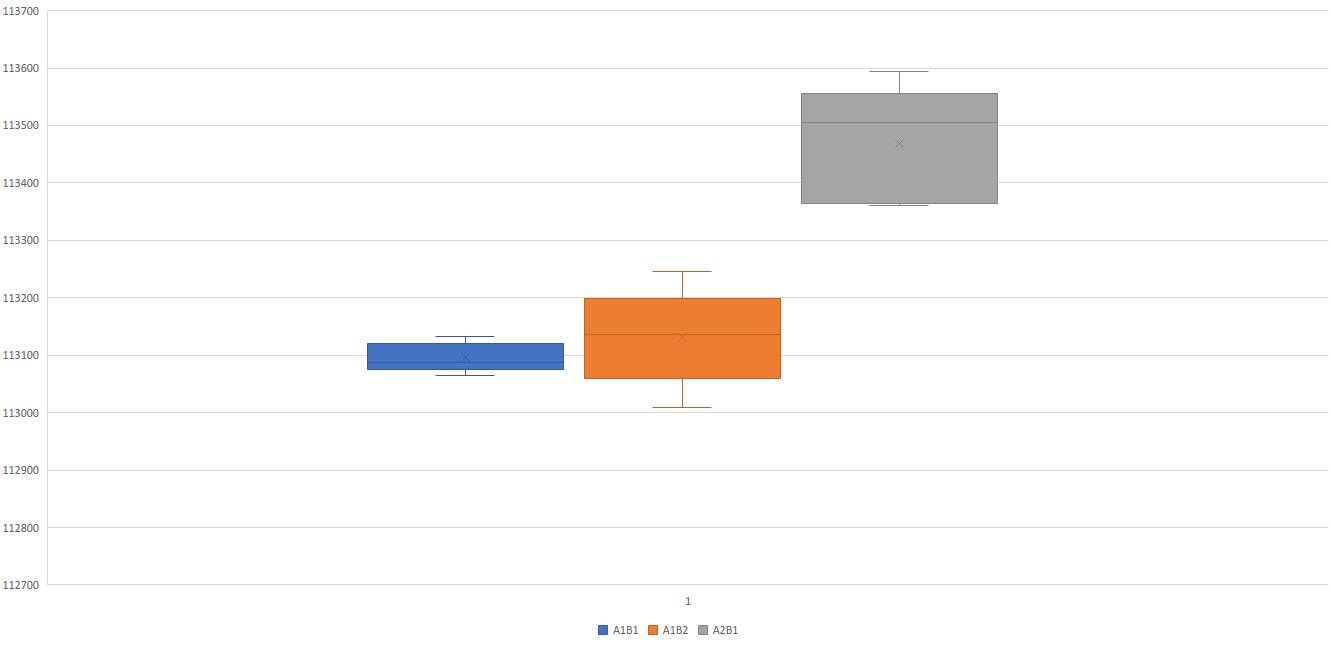
\includegraphics[scale=0.3]{img/BIGOTESMDG3.png}
		\caption{Gráfica de cajas y bigotes para el problema MDG-a23}
		\label{MDG-a23_bigotes}
	\end{figure}

	\paragraph{}En el problema MDG-a23, la configuración A1B1 obtiene muy buen resultado en cuanto a robustez de las soluciones obtenidas, seguida de A1B2 y A2B1, que obtiene la peor agrupación de resultados de las tres. En cuanto a resultados, la configuración A2B1 vuelve a ser la mejor, seguida de A1B2 y A1B1.
	
	\paragraph{}Si bien la configuración del Sistema de Colonia de Hormigas con $\alpha$=2 y $\beta$=1 en varios de los archivos de datos no consigue obtener la mejor robustez en las soluciones obtenidas, creemos que la calidad que consigue obtener respecto a estas es motivo suficiente como para considerarla la mejor configuración de las tres.
	
	\paragraph{}Si atendemos a las gráficas de convergencia del epígrafe 4.4 observamos que para las series GKD esta configuración converge ligeramente más rápido que las otras dos. Para las series SOM se evidencia aún más esta rapidez de convergencia, siendo en las series más grandes de datos, MDG, donde se observa claramente cómo la configuración elegida como ganadora obtiene una clara ventaja respecto a sus competidoras en rapidez de convergencia hacia el óptimo global.
	
	\paragraph{}Además, como tónica general, se puede apreciar en el mismo epígrafe cómo en todas las series de datos la misma configuración es capaz de empezar a encontrar soluciones con menos de 1\% de diferencia respecto al óptimo global notablemente antes que las otras dos configuraciones contrincantes.
	
	\paragraph{}De este modo, teniendo en cuenta todas las evidencias detectadas y anteriormente expuestas \textbf{elegimos como configuración ganadora el Sistema de Colonias de Hormigas con $\alpha$=2 y $\beta$=1.} 
	
	\subsubsection{Causas del mejor resultados}
	
	\paragraph{}Hemos querido explicar desde un marco teórico el porqué la configuración resultante como vencedora es capaz de obtener mejores resultados, para complementar los datos experimentales del estudio.
	
	\paragraph{}Como hemos visto en clase, los Sistemas de Colonias de Hormigas tienen un alto componente exploratorio, aunque se apliquen las mejoras introducidas respecto a los sistemas de hormigas:
	
	\begin{itemize}
		\item El equilibrio entre exploración y explotación aplicado en la regla de la transición.
		\item La actualización de la feromona solo de la mejor hormiga de la colonia y evaporación del resto de arcos del dominio del problema.
		\item Actualización local de la feromona online.
	\end{itemize}

	\paragraph{}Dentro de estas mejoras, la modificación de los valores de $\alpha$ y $\beta$ afecta directamente a la forma en la que distribuimos la probabilidad de transición de entre todos los arcos posibles:
	
	\begin{equation}
	p_{k}(r,s)= \left\lbrace
	\begin{array}{ll}
	\textup{si } q0 \leq q & \textup{arg }max_{u \in J_{k}(r)}\{(\tau_{ru})^{\alpha}*(\eta_{ru})^{\beta}\}\\
	\textup{en otro caso } & p'_{k}(r,s)
	\end{array}
	\right.
	\end{equation}
	
	\begin{equation}
	p'_{k}(r,s)= \left\lbrace
	\begin{array}{ll}
	\textup{si } s \in J_{k}(r) & \frac{(\tau_{rs})^{\alpha}*(\eta_{rs})^{\beta}}{\sum_{u \in J_{k}(r)}(\tau_{ru})^{\alpha}*(\eta_{ru})^{\beta}}\\
	\textup{en otro caso } & 0
	\end{array}
	\right.
	\end{equation}
	
	\paragraph{}Un mayor valor de $\beta$ ocasiona que los arcos con mejor coste de aporte a la solución actual reciban un mayor reparto de probabilidad, esto genera que las hormigas tiendan a guiarse por el coste de los arcos pudiendo llegar a estancarse en zonas de óptimos globales.
	
	\paragraph{}Sin embargo, un mayor valor de $\alpha$ favorece la distribución de la feromona a aquellos arcos que más feromona posean, es decir, favorece que las hormigas se desplacen a arcos que puede que no obtengan mejor aporte de solución pero que sean los más prometedores. 
	
	\paragraph{}Aquí entran en juego las dos mejoras: la actualización de la feromona solo de la mejor hormiga y la actualización de la feromona local. Como conclusión, las hormigas tienden a desplazarse a arcos por los que no han pasado hormigas y en entornos cercanos a los transitados por la mejor hormiga, obteniendo un gran equilibrio entre exploración y explotación.
	
	\subsection{Mejoras detectadas}
	
	\subsubsection{Actualización de la feromona local}
	
	\paragraph{}En la realización de las pruebas 
	
	\begin{figure}[H]
		\centering
		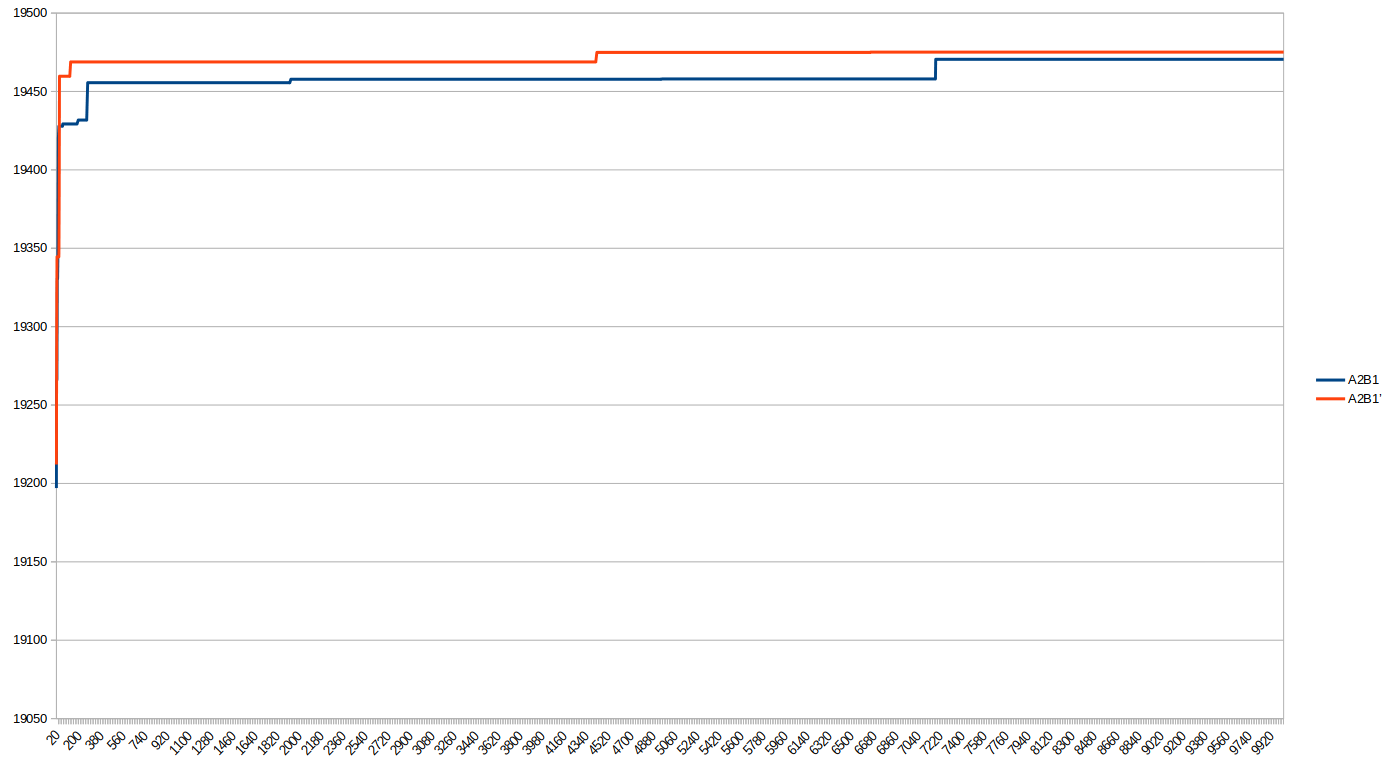
\includegraphics[scale=0.3]{img/convergenciaGKD1mejora.png}
		\caption{Evolución del mejor coste en la ejecución de la modificación para el problema GKD-c1, semilla 35608477}
		\label{gkd-c1_convergencia_mejora}
	\end{figure}

	\begin{figure}[H]
		\centering
		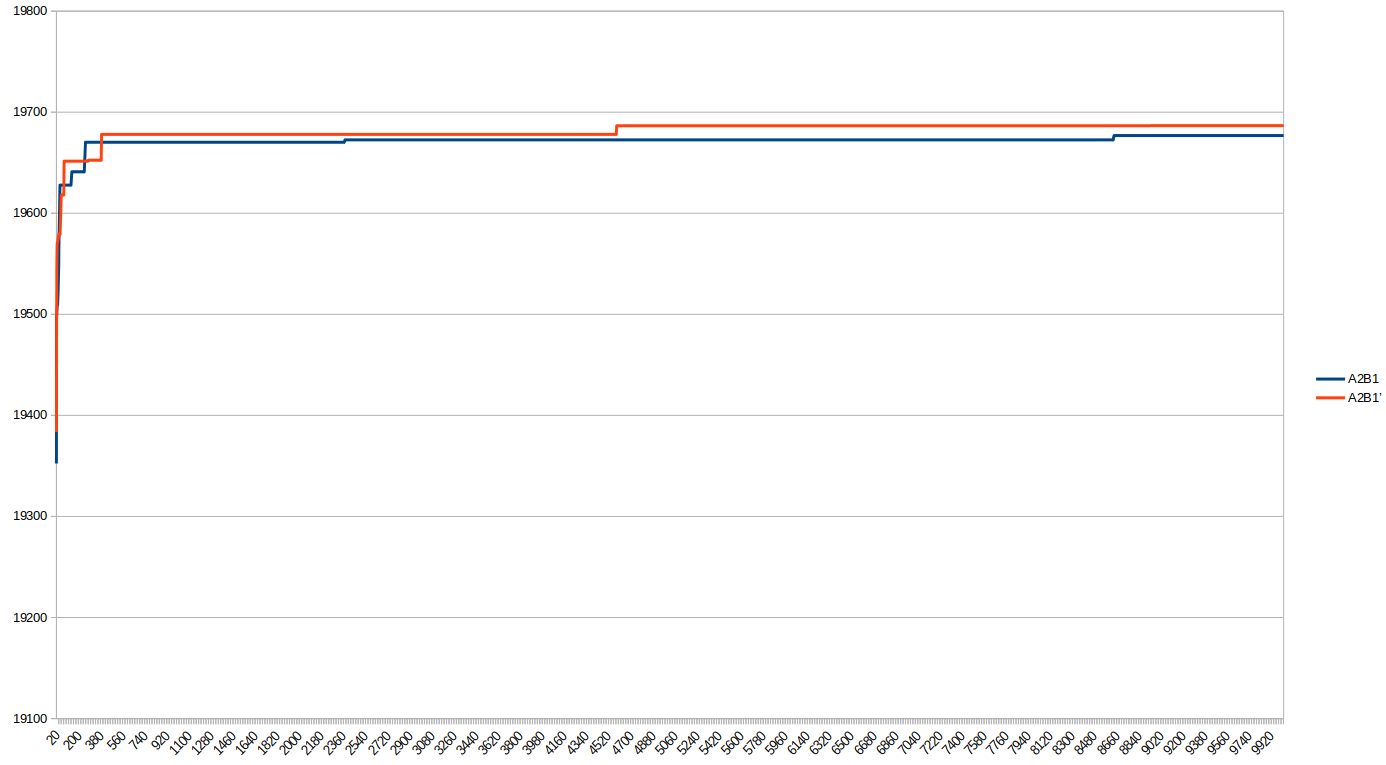
\includegraphics[scale=0.3]{img/convergenciaGKD2mejora.png}
		\caption{Evolución del mejor coste en la ejecución de la modificación para el problema GKD-c2, semilla 35608477}
		\label{gkd-c2_convergencia_mejora}
	\end{figure}

	\begin{figure}[H]
		\centering
		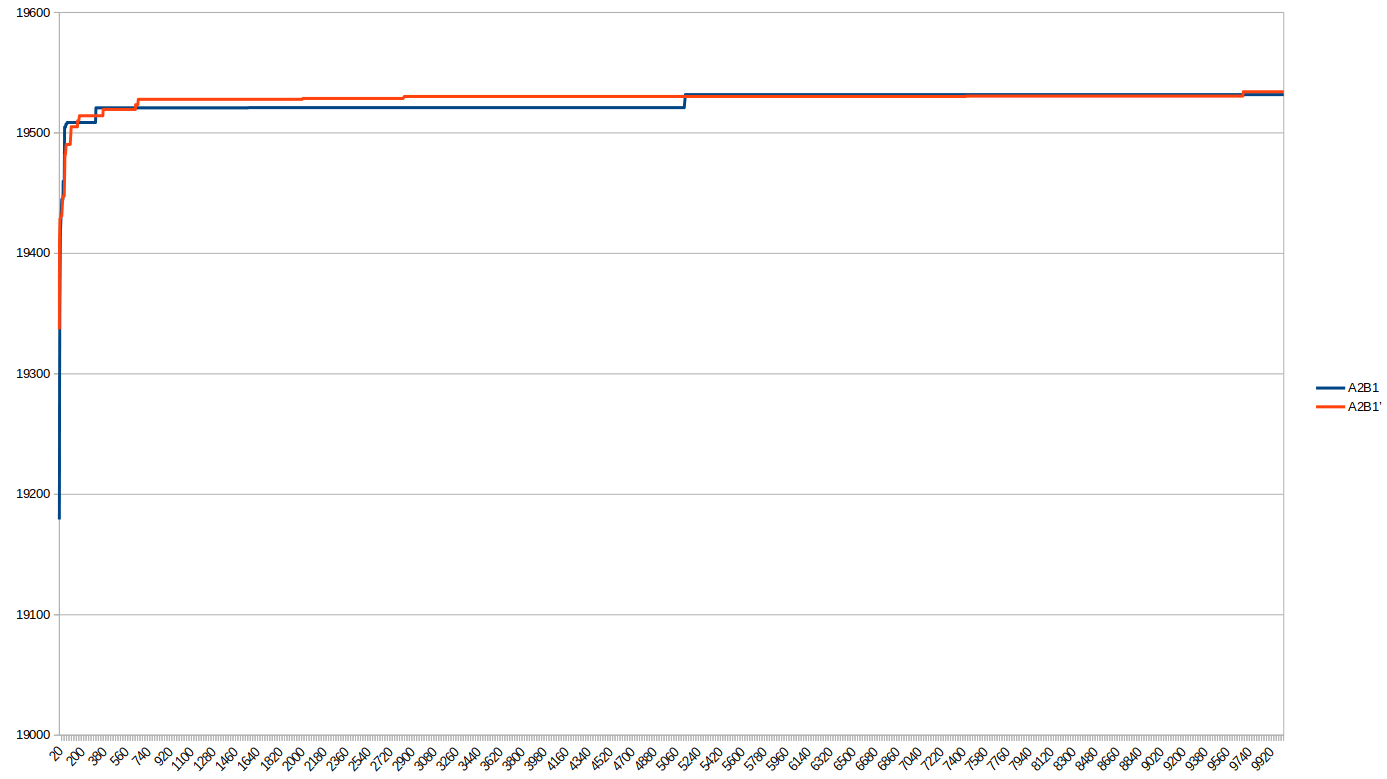
\includegraphics[scale=0.3]{img/convergenciaGKD3mejora.png}
		\caption{Evolución del mejor coste en la ejecución de la modificación para el problema GKD-c3, semilla 35608477}
		\label{gkd-c3_convergencia_mejora}
	\end{figure}

	\begin{figure}[H]
		\centering
		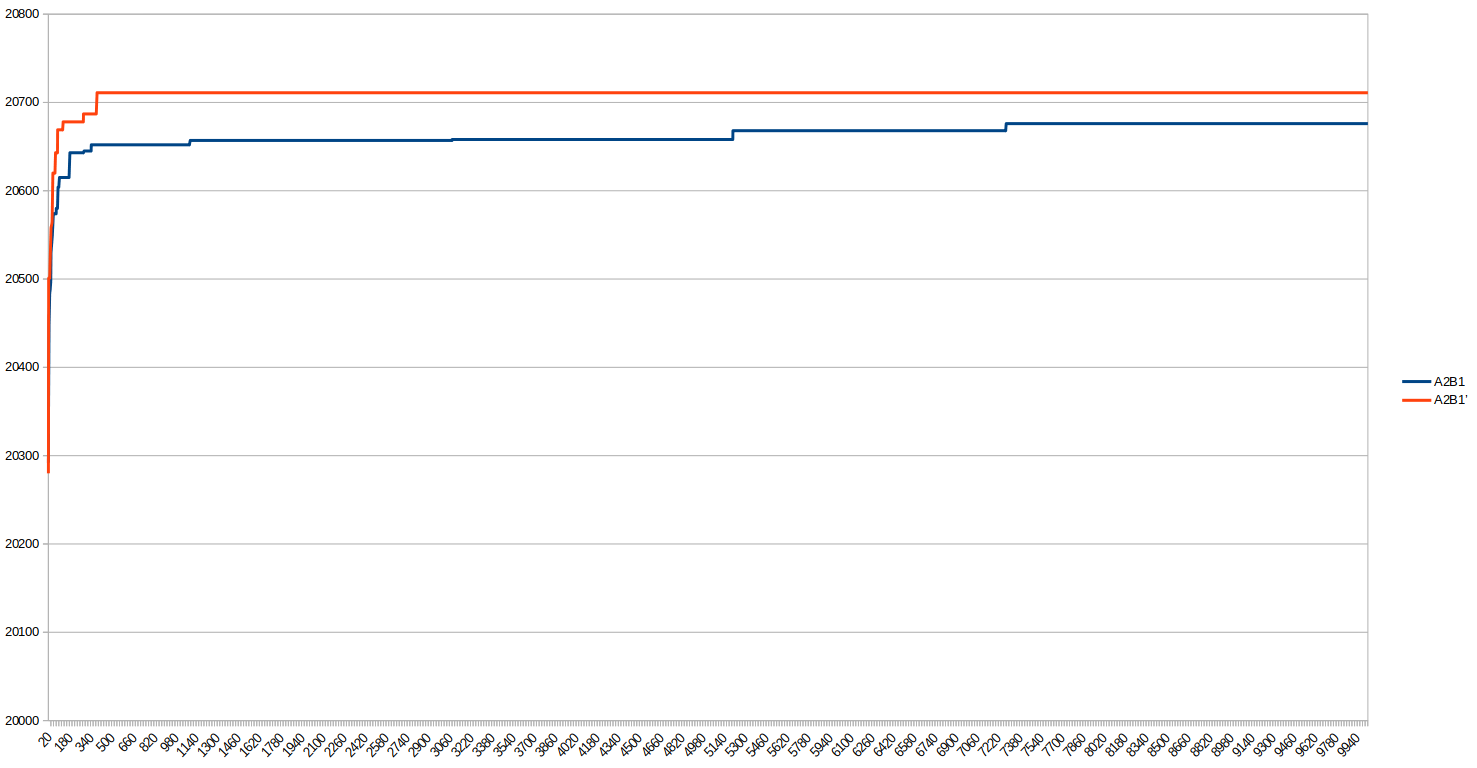
\includegraphics[scale=0.3]{img/convergenciaSOM1mejora.png}
		\caption{Evolución del mejor coste en la ejecución de la modificación para el problema SOM-b11, semilla 35608477}
		\label{SOM-b_11_convergencia_mejora}
	\end{figure}

	\begin{figure}[H]
		\centering
		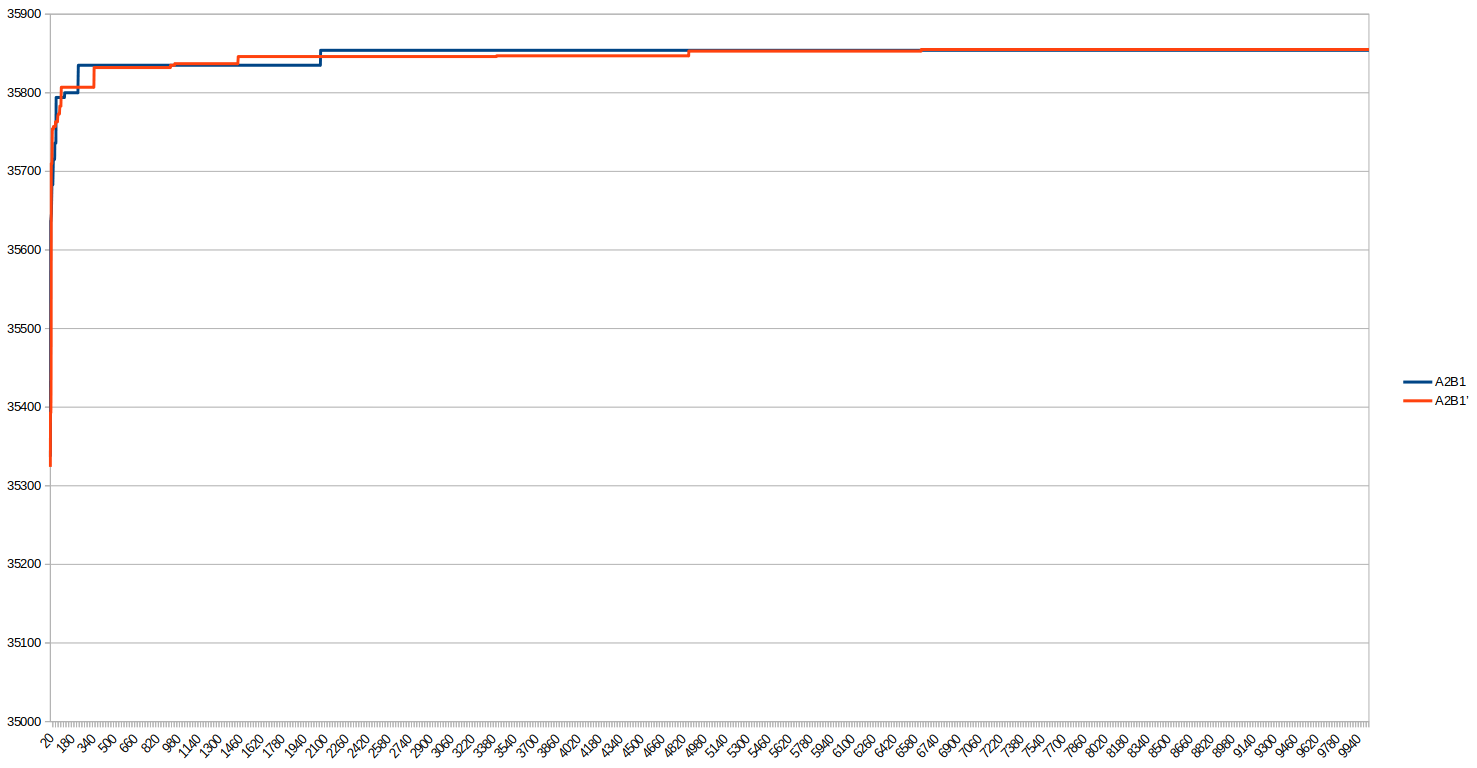
\includegraphics[scale=0.3]{img/convergenciaSOM2mejora.png}
		\caption{Evolución del mejor coste en la ejecución de la modificación para el problema SOM-b12, semilla 35608477}
		\label{SOM-b_12_convergencia_mejora}
	\end{figure}

	\begin{figure}[H]
		\centering
		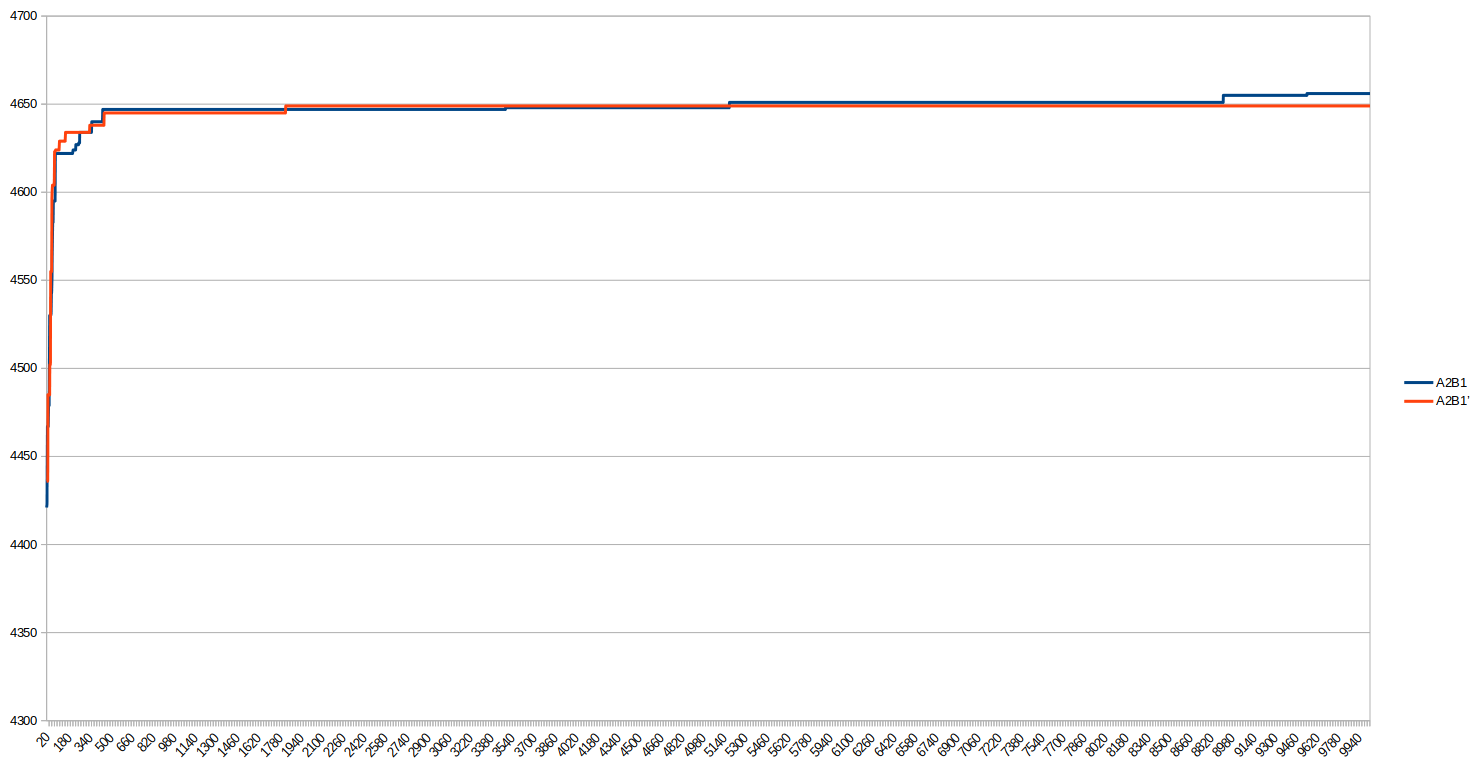
\includegraphics[scale=0.3]{img/convergenciaSOM3mejora.png}
		\caption{Evolución del mejor coste en la ejecución de la modificación para el problema SOM-b13, semilla 35608477}
		\label{SOM-b_13_convergencia_mejora}
	\end{figure}

	\begin{figure}[H]
		\centering
		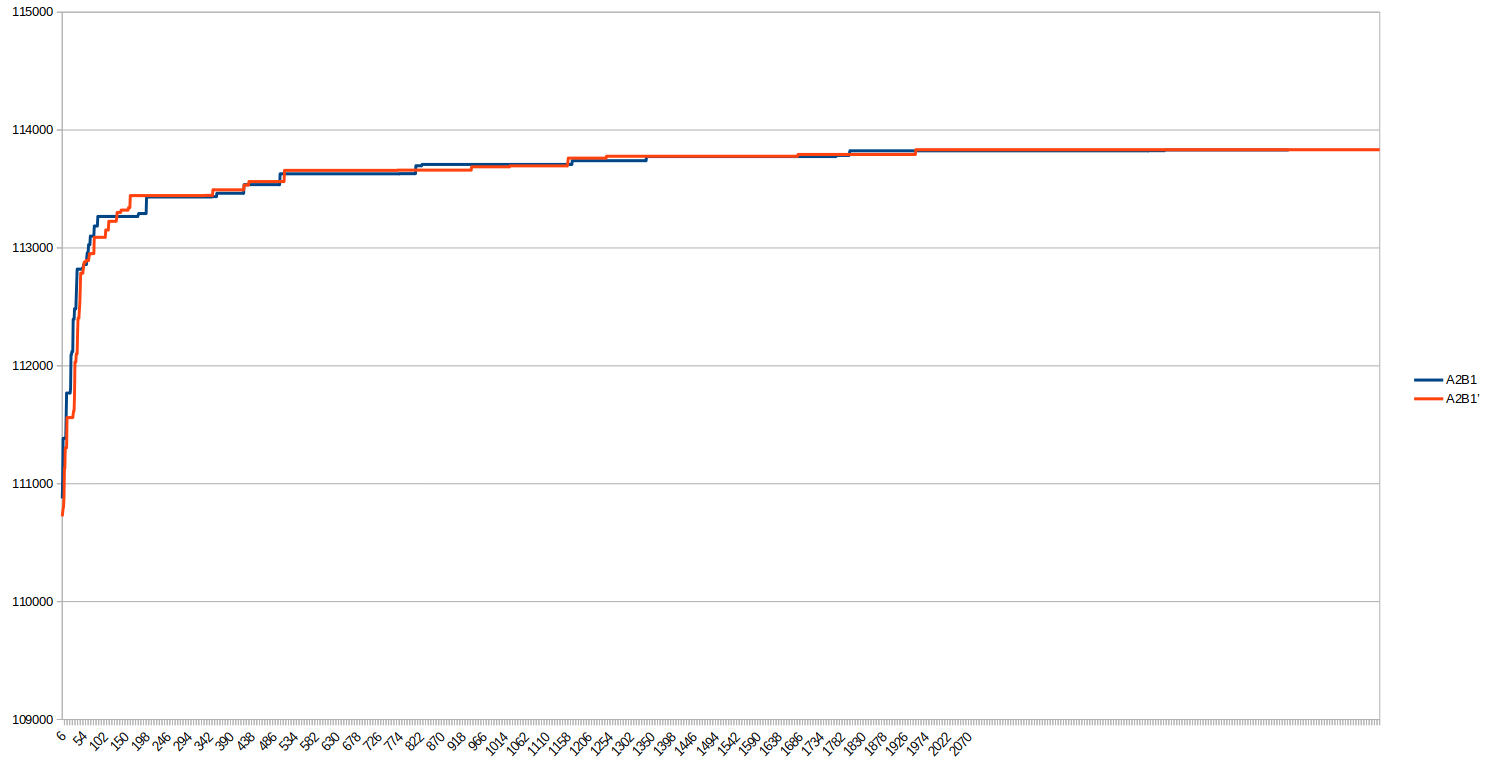
\includegraphics[scale=0.3]{img/convergenciaMDG1mejora.png}
		\caption{Evolución del mejor coste en la ejecución de la modificación para el problema MDG-a21, semilla 35608477}
		\label{MDG-a_21_convergencia_mejora}
	\end{figure}

	\begin{figure}[H]
		\centering
		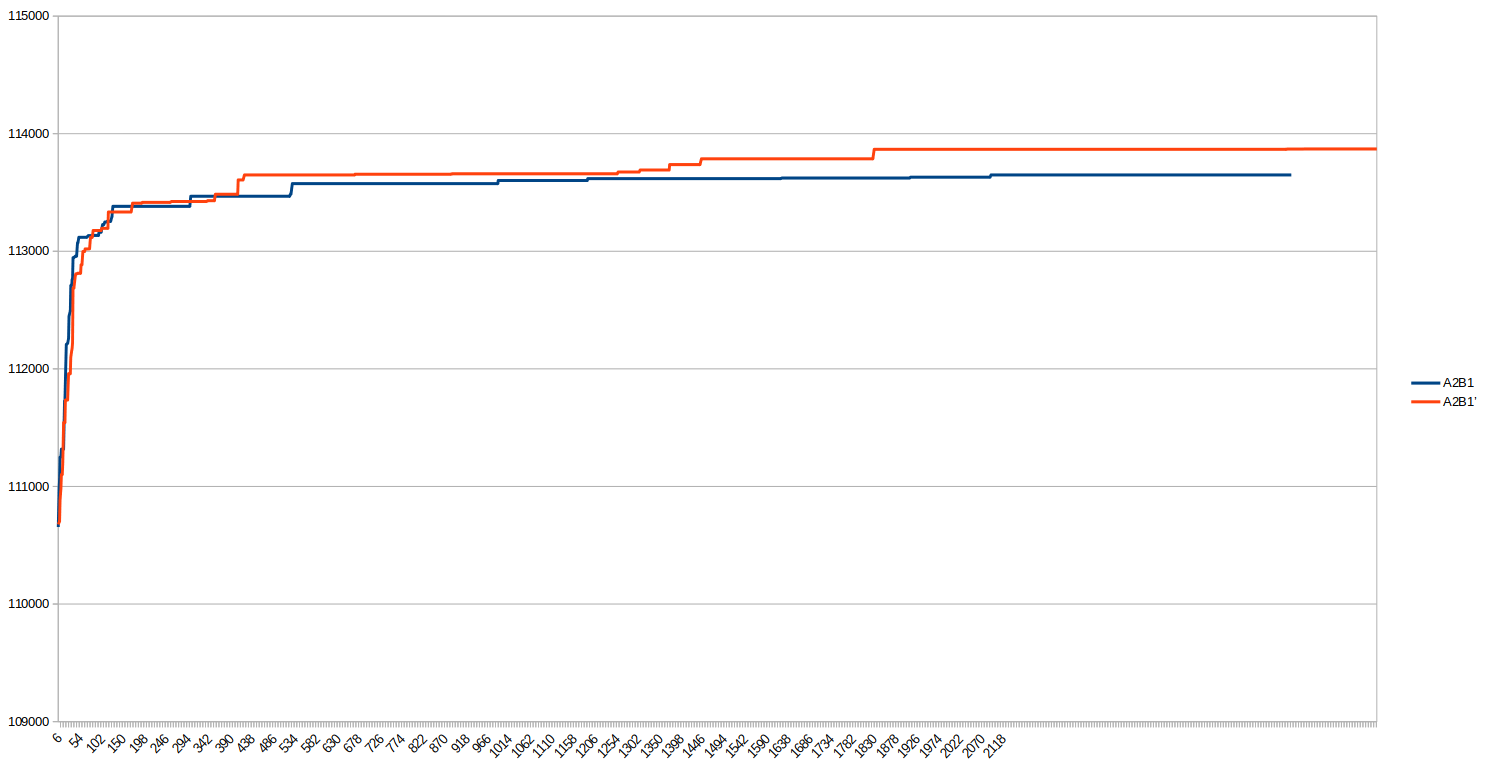
\includegraphics[scale=0.3]{img/convergenciaMDG2mejora.png}
		\caption{Evolución del mejor coste en la ejecución de la modificación para el problema MDG-a22, semilla 35608477}
		\label{MDG-a_22_convergencia_mejora}
	\end{figure}

	\begin{figure}[H]
		\centering
		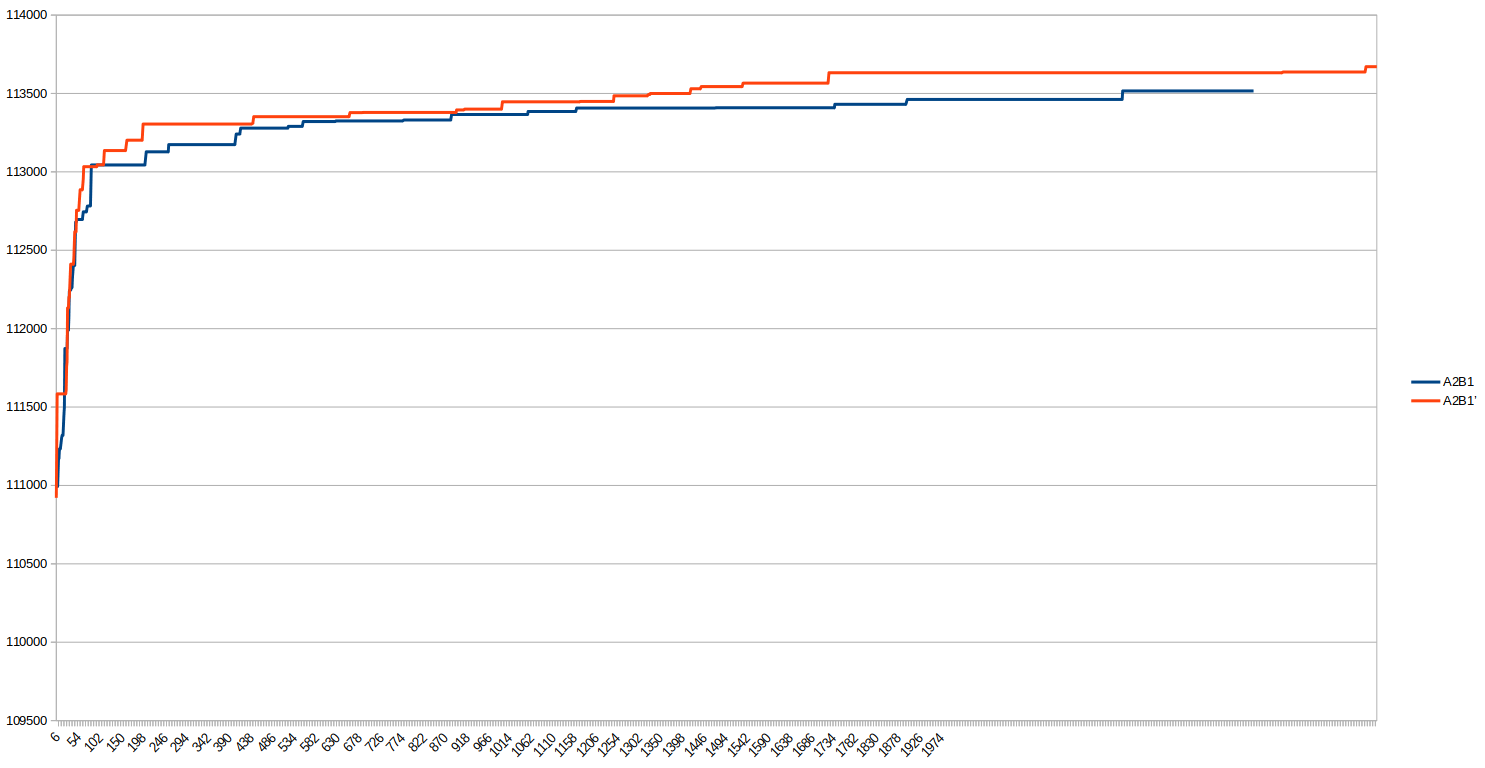
\includegraphics[scale=0.3]{img/convergenciaMDG3mejora.png}
		\caption{Evolución del mejor coste en la ejecución de la modificación para el problema MDG-a23, semilla 35608477}
		\label{MDG-a_23_convergencia_mejora}
	\end{figure}
	
	\subsubsection{Lista Restringida de Candidatos}
	
		\paragraph{} Se propone definir una LRC dinámica, aumentando el valor de $\delta$ conforme más elementos se añadan a la solución, potenciando la explotación en los últimos elementos a incorporar y favoreciendo la exploración en las primeras etapas.
	
	\subsection{Búsqueda local vs búsqueda tabú vs algoritmo genético con operador de cruce MPX elitismo 3 vs S.C.H. $\alpha$=2 $\beta$=1}
	
	\subsubsection{Resultados de la búsqueda local}
	
	\begin{table}[H]
		\begin{center}
			\begin{tabular}{| c | c | c | c | c | c | c |}
				\hline
				\multicolumn{7}{ |c| }{Búsqueda Local} \\ \hline
				& \multicolumn{2}{ |c| }{GKD-c\_1\_n500\_m50} & \multicolumn{2}{ |c| }{GKD-c\_2\_n500\_m50} & \multicolumn{2}{ |c| }{GKD-c\_3\_n500\_m50} \\ \hline
				Ejecución & Coste & Tiempo & Coste & Tiempo & Coste & Tiempo \\ \hline
				1 & 19485,188 & 75 & 19701,521 & 50 & 19542,49 & 54 \\
				2 & 19485,19  & 46 & 19701,523 & 44 & 19539,79 & 41 \\
				3 & 19485,188 & 42 & 19699,041 & 49 & 19542,49 & 53 \\
				4 & 19485,188 & 47 & 19699,848 & 49 & 19542,49 & 46 \\
				5 & 19485,188 & 37 & 19700,873 & 44 & 19542,49 & 50 \\ \hline
				Media & 0,00\% & 49,40 &0,00\% & 47,20 & -0,03\% & 48,80 \\ \hline
				Devs. típica & 0,00\% & 14,84 & 0,01\% & 2,95  &0,01\% & 5,36\\ \hline
			\end{tabular}
			\caption{Resultados GKD}
			\label{tab:tabGKDLOCAL}
		\end{center}
	\end{table} 
	
	
	\begin{table}[H]
		\begin{center}
			\begin{tabular}{| c | c | c | c | c | c | c |}
				\hline
				\multicolumn{7}{ |c| }{Búsqueda Local} \\ \hline
				& \multicolumn{2}{ |c| }{SOM-b\_11\_n300\_m90} & \multicolumn{2}{ |c| }{SOM-b\_12\_n300\_m120} & \multicolumn{2}{ |c| }{SOM-b\_13\_n400\_m40} \\ \hline
				Ejecución & Coste & Tiempo & Coste & Tiempo & Coste & Tiempo\\\hline
				1 & 20720 & 33 & 35856 & 34 & 4482 & 15 \\
				2 & 20622 & 29 & 35771 & 41 & 4542 & 19 \\
				3 & 20594 & 32 & 35758 & 43 & 4553 & 20 \\
				4 & 20652 & 35 & 35740 & 39 & 4545 & 20 \\
				5 & 20612 & 152 & 35767 & 41 & 4506 & 16 \\ \hline
				Media &-0,50\% & 56,20 &-0,29\% & 39,60 &-2,84\% & 18,00\\ \hline
				Devs. típica &0,24\% & 53,60 &0,13\% & 3,44 &0,65\% & 2,35\\ \hline
			\end{tabular}
			\caption{Resultados SOM}
			\label{tab:tabSOMLOCAL}
		\end{center}
	\end{table} 
	
	\begin{table}[H]
		\begin{center}
			\begin{tabular}{| c | c | c | c | c | c | c |}
				\hline
				\multicolumn{7}{ |c| }{Búsqueda Local} \\ \hline
				& \multicolumn{2}{ |c| }{MDG-a\_21\_n2000\_m200} & \multicolumn{2}{ |c| }{MDG-a\_22\_n2000\_m200} & \multicolumn{2}{ |c| }{MDG-a\_23\_n2000\_m200}\\\hline
				Ejecución & Coste & Tiempo & Coste & Tiempo & Coste & Tiempo\\\hline
				1 & 112638 & 895 & 112923 & 1472 & 113333 & 1125\\
				2 & 112829 & 847 & 113382 & 1127 & 112874 & 1630\\
				3 & 112945 & 943 & 112724 & 1293 & 112952 & 1015\\
				4 & 113286 & 2224 & 113162 & 1123 & 113147 & 1709\\
				5 & 113141 & 2731 & 112973 & 1055 & 113131 & 1047\\ \hline
				Media &-1,13 \% & 1528,00 &-1,13\% & 1214,00 & -0,91\% & 1305,20\\ \hline
				Devs. típica & 0,22\% & 885,76 & 0,22\% & 168,77 & 0,16\% & 336,12\\ \hline
			\end{tabular}
			\caption{Resultados MDG}
			\label{tab:tabMDGLOCAL}
		\end{center}
	\end{table}
	
	
	
	\subsubsection{Resultados de la búsqueda tabú}
	
	\begin{table}[H]
		\begin{center}
			\begin{tabular}{| c | c | c | c | c | c | c |}
				\hline
				\multicolumn{7}{ |c| }{Búsqueda Tabú} \\ \hline
				& \multicolumn{2}{ |c| }{GKD-c\_1\_n500\_m50} & \multicolumn{2}{ |c| }{GKD-c\_2\_n500\_m50} & \multicolumn{2}{ |c| }{GKD-c\_3\_n500\_m50} \\ \hline
				Ejecución & Coste & Tiempo & Coste & Tiempo & Coste & Tiempo \\ \hline
				1 & 19485,184 & 1900 & 19701,521 & 1723 & 19547,215 & 1699 \\
				2 & 19485,184 & 1790 & 19701,521 & 1717 & 19547,215 & 1968\\
				3 & 19485,188 & 1734 & 19701,521 & 1715 & 19547,215 & 1717\\
				4 & 19485,19  & 1710 & 19701,523 & 1786 & 19547,215 & 1705\\
				5 & 19485,184 & 1700 & 19701,521 & 2041 & 19547,215 & 1693\\ \hline
				Media & 0,00\% & 1766,80 &0,00\% & 1796,40 & 0,00\% & 1756,40
				 \\ \hline
				Devs. típica & 0,00\% & 82,23 & 0,00\% & 139,87 &0,00\% & 118,62 \\ \hline
			\end{tabular}
			\caption{Resultados GKD}
			\label{tab:tabGKDTABU}
		\end{center}
	\end{table} 
	
	
	\begin{table}[H]
		\begin{center}
			\begin{tabular}{| c | c | c | c | c | c | c |}
				\hline
				\multicolumn{7}{ |c| }{Búsqueda Tabú} \\ \hline
				& \multicolumn{2}{ |c| }{SOM-b\_11\_n300\_m90} & \multicolumn{2}{ |c| }{SOM-b\_12\_n300\_m120} & \multicolumn{2}{ |c| }{SOM-b\_13\_n400\_m40} \\ \hline
				Ejecución & Coste & Tiempo & Coste & Tiempo & Coste & Tiempo\\\hline
				1 & 20705 & 5362 & 35881 & 11727 & 4654 & 1069 \\
				2 & 20732 & 6174 & 35881 & 11616 & 4658 & 1072 \\
				3 & 20731 & 5345 & 35881 & 11665 & 4644 & 1075 \\
				4 & 20725 & 5278 & 35881 & 11676 & 4627 & 1066 \\
				5 & 20735 & 5718 & 35881 & 11611 & 4634 & 1109 \\ \hline
				Media &-0,08\% & 5575,40 &0,00\% & 11659,00 &-0,31\% & 1078,20 \\ \hline
				Devs. típica &0,06\% & 376,07 &0,00\% & 47,70 &0,28\% & 17,54 \\ \hline
			\end{tabular}
			\caption{Resultados SOM}
			\label{tab:tabSOMTABU}
		\end{center}
	\end{table} 
	
	\begin{table}[H]
		\begin{center}
			\begin{tabular}{| c | c | c | c | c | c | c |}
				\hline
				\multicolumn{7}{ |c| }{Búsqueda Tabú} \\ \hline
				& \multicolumn{2}{ |c| }{MDG-a\_21\_n2000\_m200} & \multicolumn{2}{ |c| }{MDG-a\_22\_n2000\_m200} & \multicolumn{2}{ |c| }{MDG-a\_23\_n2000\_m200}\\\hline
				Ejecución & Coste & Tiempo & Coste & Tiempo & Coste & Tiempo\\\hline
				1 & 113613 & 51002 & 113697 & 51713 & 113429 & 51636\\
				2 & 113199 & 51021 & 113306 & 51397 & 113517 & 51131\\
				3 & 113831 & 51184 & 113329 & 51482 & 113540 & 51819\\
				4 & 113565 & 50643 & 113414 & 51179 & 113385 & 51073\\
				5 & 113647 & 51279 & 113396 & 51037 & 113693 & 51224\\ \hline
				Media &-0,60 \% & 50825,80 &-0,79\% & 51361,60 & -0,53\% & 51376,60 \\ \hline
				Devs. típica & 0,20\% & 511,34 & 0,14\% & 263,60 & 0,10\% & 331,20 \\ \hline
			\end{tabular}
			\caption{Resultados MDG}
			\label{tab:tabMDGTABU}
		\end{center}
	\end{table}
	
	\subsubsection{Resultados del algoritmo genético con elitismo = 3}
	
	\begin{table}[H]
		\begin{center}
			\begin{tabular}{| c | c | c | c | c | c | c |}
				\hline
				\multicolumn{7}{ |c| }{Genético MPX elite 3} \\ \hline
				& \multicolumn{2}{ |c| }{GKD-c\_1\_n500\_m50} & \multicolumn{2}{ |c| }{GKD-c\_2\_n500\_m50} & \multicolumn{2}{ |c| }{GKD-c\_3\_n500\_m50} \\ \hline
				Ejecución & Coste & Tiempo & Coste & Tiempo & Coste & Tiempo \\ \hline
				1 &19481,69 & 642 & 19701,52 & 361 & 19547,22 & 348\\
				2 &19482,37 & 388 & 19701,52 & 367 & 19547,22 & 357\\
				3 &19485,19 & 366 & 19701,52 & 356 & 19547,22 & 362\\
				4 &19485,19 & 374 & 19699,48 & 351 & 19547,22 & 356\\
				5 &19485,19 & 366 & 19701,52 & 358 & 19543,48 & 358\\ \hline
				Media &0,00\% & 427,20 & 0,00\% & 358,60 & 0,00\% & 356,20 \\ \hline
				Devs. típica & 0,01\%	& 120,41 & 0,00\% & 5,94 & 0,01\% & 5,12 \\ \hline
			\end{tabular}
			\caption{Resultados GKD}
			\label{tab:tabMPXE3GKD}
		\end{center}
	\end{table} 
	
	
	\begin{table}[H]
		\begin{center}
			\begin{tabular}{| c | c | c | c | c | c | c |}
				\hline
				\multicolumn{7}{ |c| }{Genético MPX elite 3} \\ \hline
				& \multicolumn{2}{ |c| }{SOM-b\_11\_n300\_m90} & \multicolumn{2}{ |c| }{SOM-b\_12\_n300\_m120} & \multicolumn{2}{ |c| }{SOM-b\_13\_n400\_m40} \\ \hline
				Ejecución & Coste & Tiempo & Coste & Tiempo & Coste & Tiempo\\\hline
				1 &20648 & 848 & 35870 & 1533 & 4590 & 262\\
				2 &20731 & 845 & 35866 & 1466 & 4625 & 266\\
				3 &20650 & 819 & 35834 & 1525 & 4584 & 261\\
				4 &20672 & 842 & 35879 & 1482 & 4553 & 265\\
				5 &20647 & 840 & 35825 & 2266 & 4578 & 262\\\hline
				Media &-0,35\% & 848,00 & -0,07\% & 1654,40 & -1,55\% & 263,20 \\ \hline
				Devs. típica & 0,17\%	& 11,48 & 0,07\% & 343,06 & 0,56\% & 2,17 \\ \hline
			\end{tabular}
			\caption{Resultados SOM}
			\label{tab:tabMPXE3SOM}
		\end{center}
	\end{table} 
	
	\begin{table}[H]
		\begin{center}
			\begin{tabular}{| c | c | c | c | c | c | c |}
				\hline
				\multicolumn{7}{ |c| }{Genético MPX elite 3} \\ \hline
				& \multicolumn{2}{ |c| }{MDG-a\_21\_n2000\_m200} & \multicolumn{2}{ |c| }{MDG-a\_22\_n2000\_m200} & \multicolumn{2}{ |c| }{MDG-a\_23\_n2000\_m200}\\\hline
				Ejecución & Coste & Tiempo & Coste & Tiempo & Coste & Tiempo\\\hline
				1 &112931 & 8904 & 113173 & 8865 & 112978 & 8823\\
				2 &113375 & 9597 & 113335 & 8566 & 113350 & 8614\\
				3 &113193 & 9058 & 113402 & 8898 & 113212 & 8660\\
				4 &113074 & 8956 & 112677 & 8093 & 113274 & 8448\\
				5 &113445 & 8814 & 113470 & 9081 & 112600 & 8476\\\hline
				Media &-0,92\% & 9065,80 & -0,98\% & 8500,60 & -0,91\% & 8604,20 \\ \hline
				Devs. típica & 0,19\%	& 309,79 & 0,28\% & 399,12 & 0,27\% & 151,59 \\ \hline
			\end{tabular}
			\caption{Resultados MDG}
			\label{tab:tabMPXE3MDG}
		\end{center}
	\end{table}
	

	\subsubsection{Comparación de resultados}
	
	\begin{figure}[H]
		\centering
		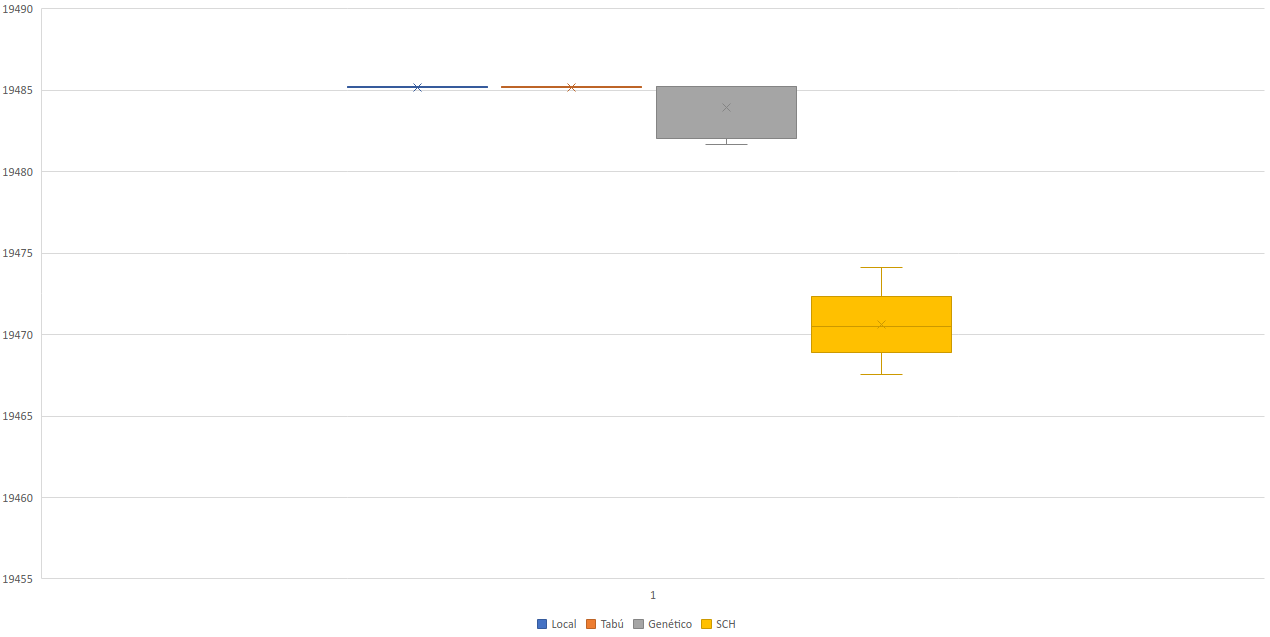
\includegraphics[scale=0.3]{img/finalGKD1.png}
		\caption{Gráfica de cajas y bigotes comparativas GKD-c1}
		\label{GKD-c1_final}
	\end{figure}

	\begin{figure}[H]
		\centering
		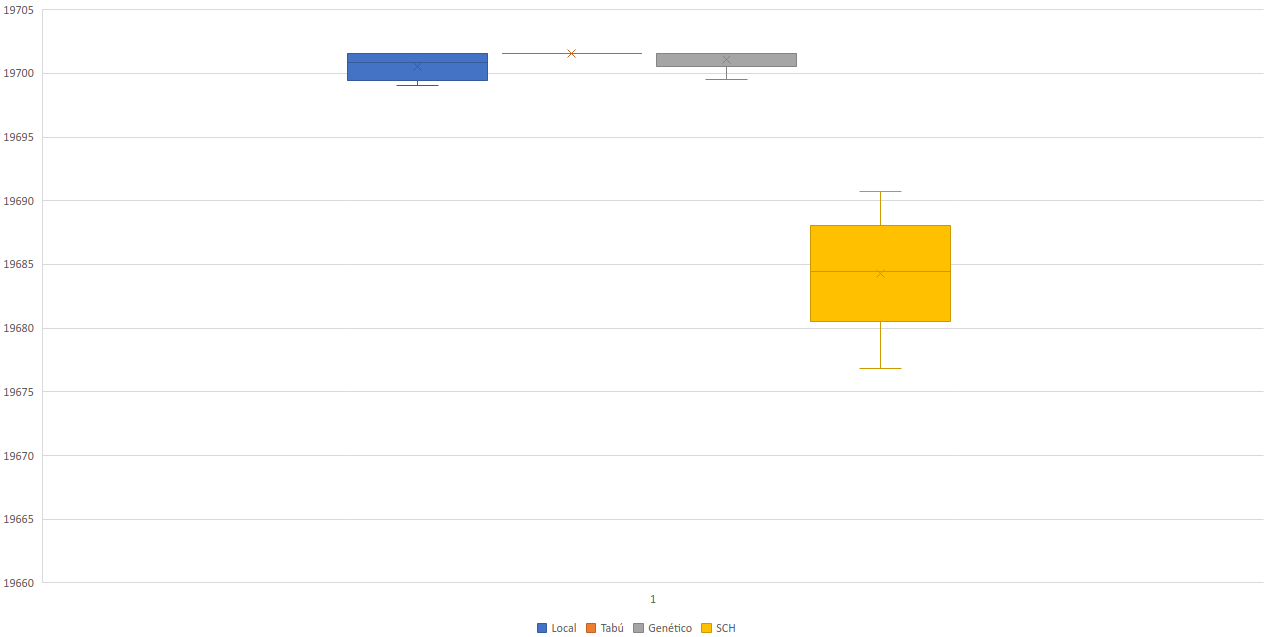
\includegraphics[scale=0.3]{img/finalGKD2.png}
		\caption{Gráfica de cajas y bigotes comparativas GKD-c2}
		\label{GKD-c2_final}
	\end{figure}

	\begin{figure}[H]
		\centering
		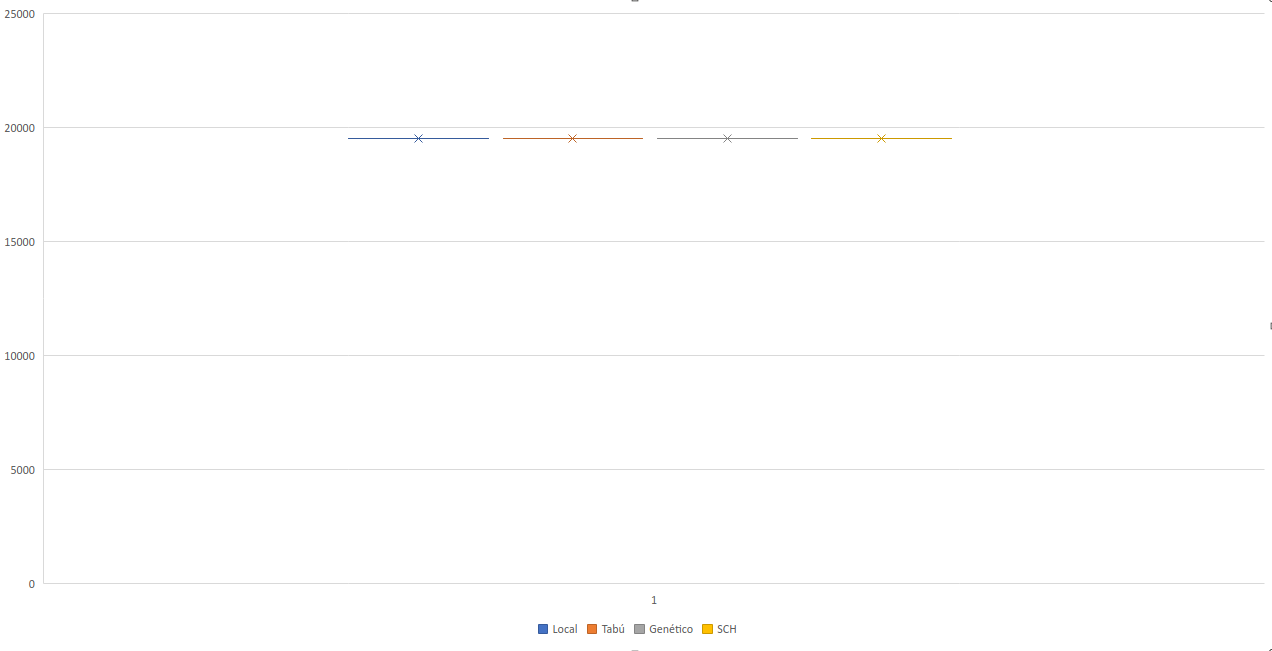
\includegraphics[scale=0.3]{img/finalGKD3.png}
		\caption{Gráfica de cajas y bigotes comparativas GKD-c3}
		\label{GKD-c3_final}
	\end{figure}

	\begin{figure}[H]
		\centering
		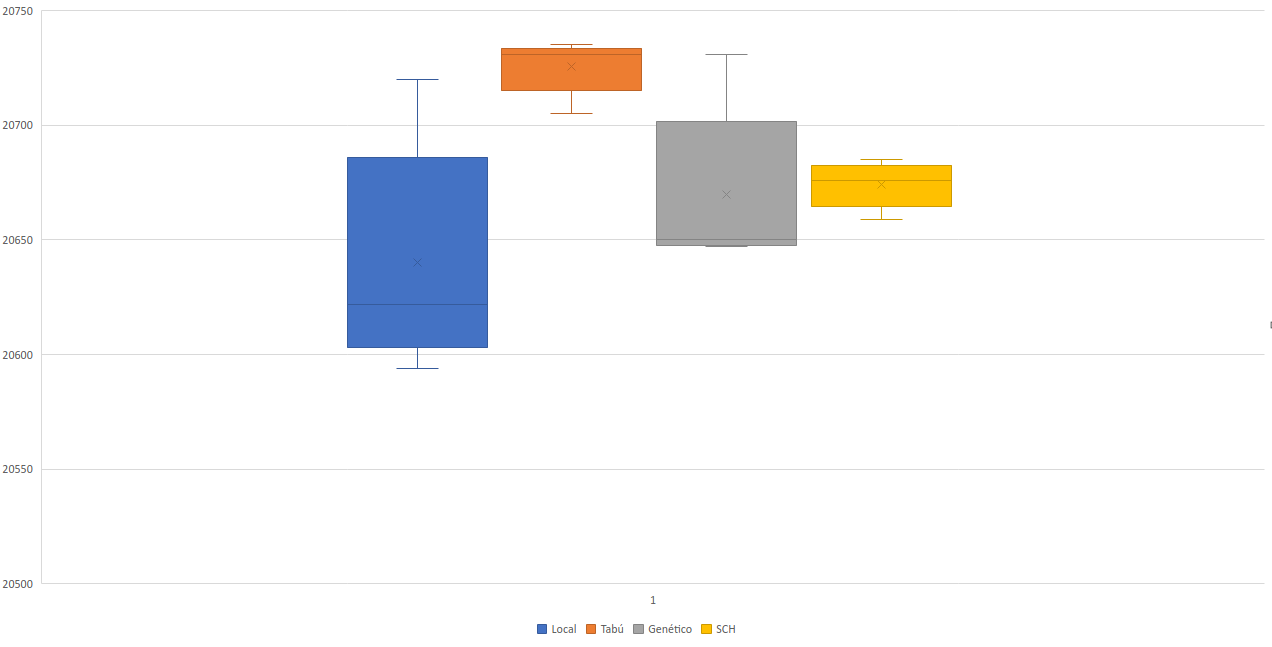
\includegraphics[scale=0.3]{img/finalSOM1.png}
		\caption{Gráfica de cajas y bigotes comparativas SOM-b11}
		\label{SOM-b11_final}
	\end{figure}

	\begin{figure}[H]
		\centering
		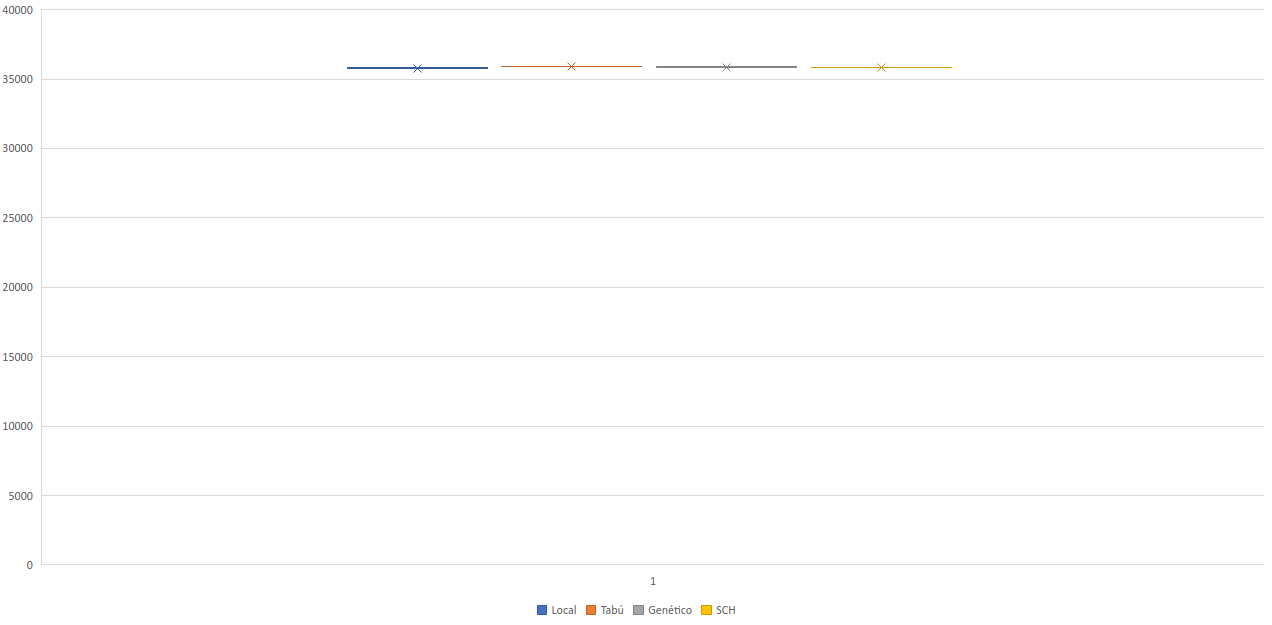
\includegraphics[scale=0.3]{img/finalSOM2.png}
		\caption{Gráfica de cajas y bigotes comparativas SOM-b12}
		\label{SOM-b12_final}
	\end{figure}

	\begin{figure}[H]
		\centering
		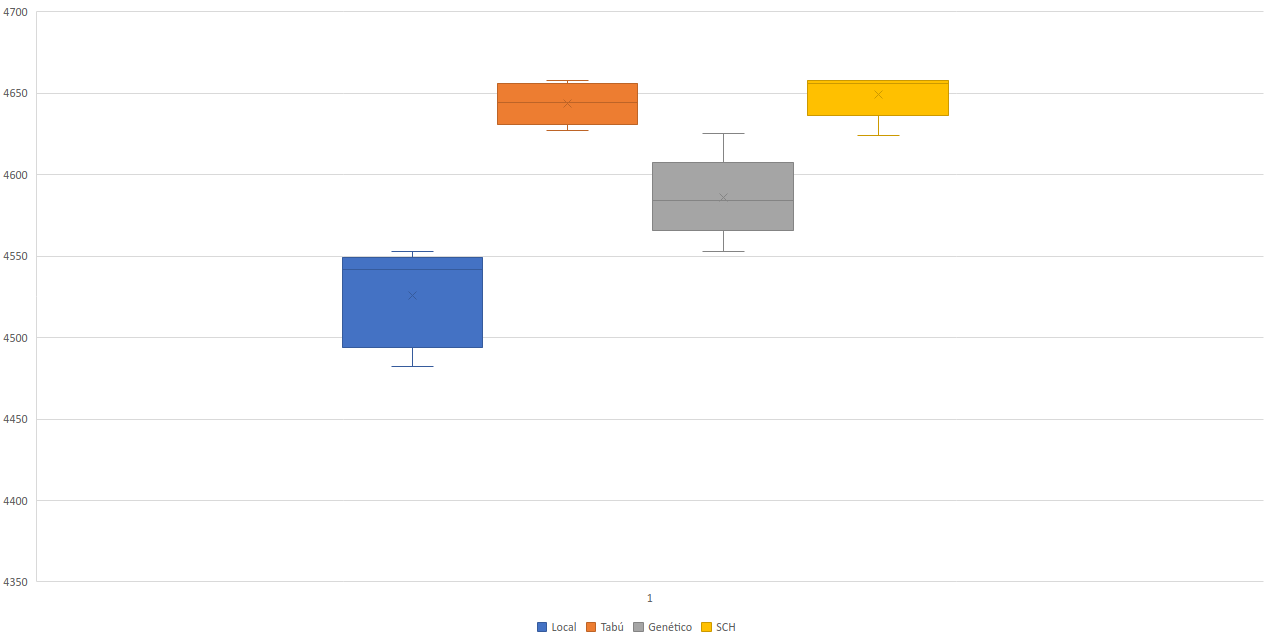
\includegraphics[scale=0.3]{img/finalSOM3.png}
		\caption{Gráfica de cajas y bigotes comparativas SOM-b13}
		\label{SOM-b13_final}
	\end{figure}

	\begin{figure}[H]
		\centering
		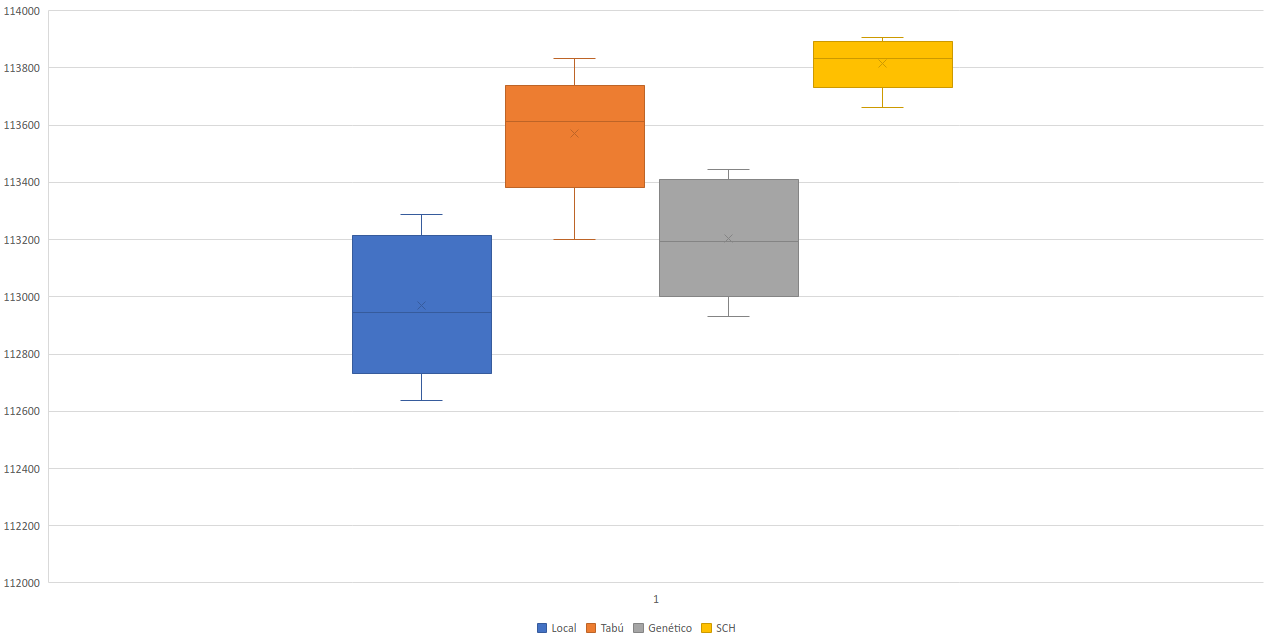
\includegraphics[scale=0.3]{img/finalMDG1.png}
		\caption{Gráfica de cajas y bigotes comparativas MDG-a21}
		\label{MDG-a21_final}
	\end{figure}

	\begin{figure}[H]
		\centering
		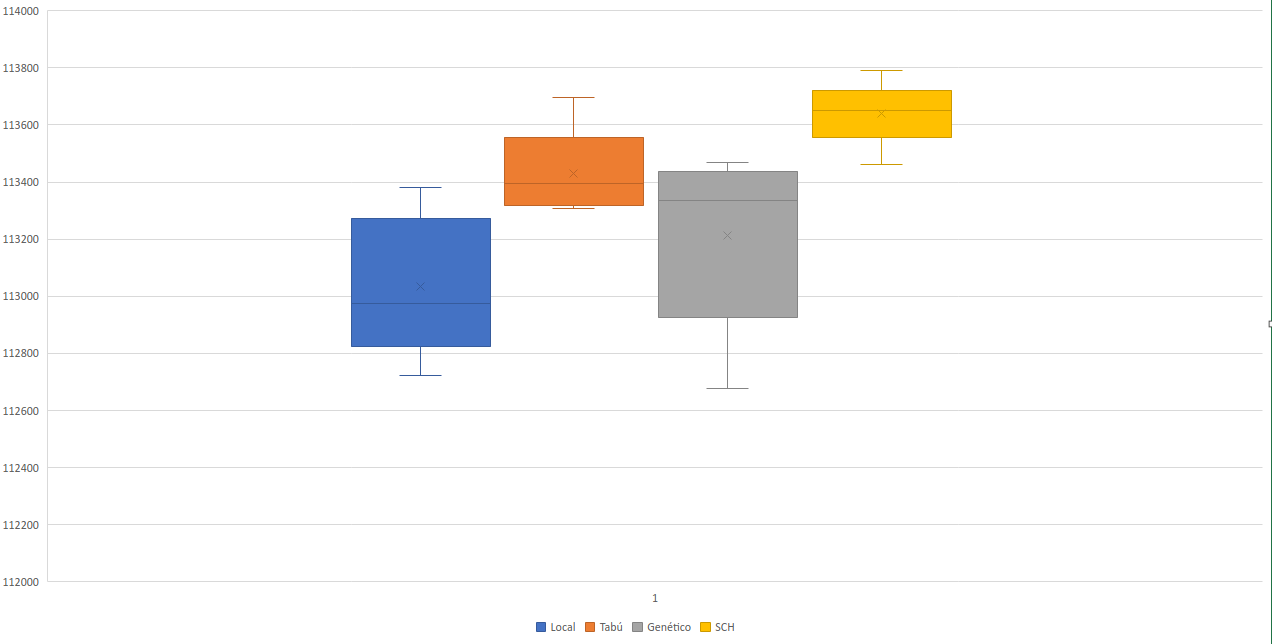
\includegraphics[scale=0.3]{img/finalMDG2.png}
		\caption{Gráfica de cajas y bigotes comparativas MDG-a22}
		\label{MDG-a22_final}
	\end{figure}

	\begin{figure}[H]
		\centering
		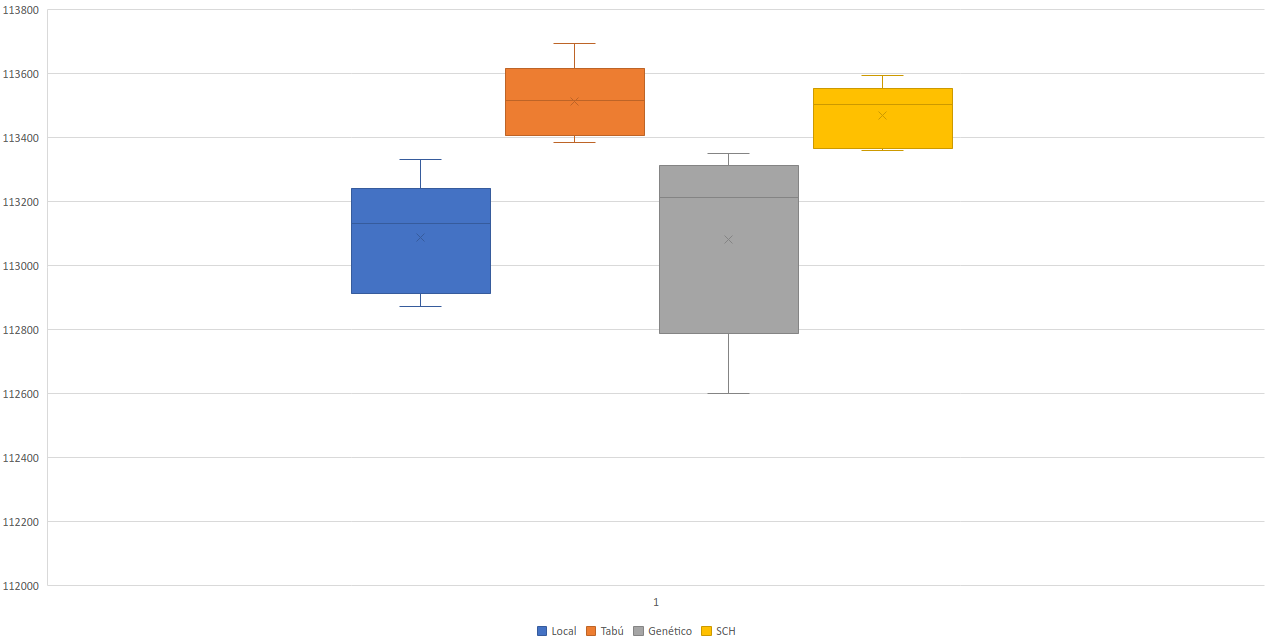
\includegraphics[scale=0.3]{img/finalMDG3.png}
		\caption{Gráfica de cajas y bigotes comparativas MDG-a23}
		\label{MDG-a23_final}
	\end{figure}
	
	\subsubsection{Conclusiones}